\documentclass{article}
\usepackage{neurips_2026} % default option: anonymous submission build (no final/preprint)

\usepackage[utf8]{inputenc}
\usepackage[T1]{fontenc}
\usepackage{hyperref}
\usepackage{url}
\usepackage{booktabs}
\usepackage{amsfonts}
\usepackage{amsmath}
\usepackage{nicefrac}
\usepackage{microtype}
\usepackage{xcolor}
\usepackage{graphicx}

\title{How Much of a Tuned Score Survives on Fresh Items? Optimism and Reliable Reporting for Automatically Tuned Prompts and Pipelines}

\author{Anonymous Author(s)}

% generated by paper/quote_numbers.py from results/*.csv; do not edit. Use as \N{key}.
\newcommand{\N}[1]{\csname num@#1\endcsname}
\expandafter\gdef\csname num@cmp_001_1616_false\endcsname{0.0}
\expandafter\gdef\csname num@cmp_001_6401_claim\endcsname{53}
\expandafter\gdef\csname num@cmp_001_6401_diff\endcsname{6.7}
\expandafter\gdef\csname num@cmp_001_6401_false\endcsname{12}
\expandafter\gdef\csname num@cmp_00_1616_false\endcsname{0.0}
\expandafter\gdef\csname num@cmp_00_6401_claim\endcsname{49}
\expandafter\gdef\csname num@cmp_00_6401_diff\endcsname{6.2}
\expandafter\gdef\csname num@cmp_00_6401_false\endcsname{20}
\expandafter\gdef\csname num@cmp_00_6401_fc05\endcsname{46}
\expandafter\gdef\csname num@cmp_00_6401_ws\endcsname{20}
\expandafter\gdef\csname num@cmp_0_6401_claim_split\endcsname{6}
\expandafter\gdef\csname num@cmp_reps\endcsname{500}
\expandafter\gdef\csname num@cov_K128\endcsname{46}
\expandafter\gdef\csname num@cov_K16\endcsname{76}
\expandafter\gdef\csname num@cov_K2\endcsname{95}
\expandafter\gdef\csname num@cov_K32\endcsname{69}
\expandafter\gdef\csname num@cov_K4\endcsname{91}
\expandafter\gdef\csname num@cov_K64\endcsname{56}
\expandafter\gdef\csname num@cov_K8\endcsname{85}
\expandafter\gdef\csname num@cov_greedy\endcsname{76}
\expandafter\gdef\csname num@cov_leak3\endcsname{64}
\expandafter\gdef\csname num@cov_leak8\endcsname{41}
\expandafter\gdef\csname num@cov_n100\endcsname{77}
\expandafter\gdef\csname num@cov_n1000\endcsname{85}
\expandafter\gdef\csname num@cov_n200\endcsname{76}
\expandafter\gdef\csname num@cov_n2000\endcsname{86}
\expandafter\gdef\csname num@cov_n50\endcsname{75}
\expandafter\gdef\csname num@cov_n500\endcsname{79}
\expandafter\gdef\csname num@cov_sh\endcsname{86}
\expandafter\gdef\csname num@cov_sr\endcsname{69}
\expandafter\gdef\csname num@fp_K128\endcsname{54}
\expandafter\gdef\csname num@fp_leak3\endcsname{34}
\expandafter\gdef\csname num@fp_leak8\endcsname{53}
\expandafter\gdef\csname num@fr_boot_632_200_bias\endcsname{1.6}
\expandafter\gdef\csname num@fr_boot_632_200_cover\endcsname{96}
\expandafter\gdef\csname num@fr_boot_632_200_mu\endcsname{30.5}
\expandafter\gdef\csname num@fr_boot_632_200_rmse\endcsname{3.1}
\expandafter\gdef\csname num@fr_boot_632_200_width\endcsname{12.9}
\expandafter\gdef\csname num@fr_boot_632_400_bias\endcsname{1.1}
\expandafter\gdef\csname num@fr_boot_632_400_cover\endcsname{96}
\expandafter\gdef\csname num@fr_boot_632_400_mu\endcsname{30.6}
\expandafter\gdef\csname num@fr_boot_632_400_rmse\endcsname{2.3}
\expandafter\gdef\csname num@fr_boot_632_400_width\endcsname{9.1}
\expandafter\gdef\csname num@fr_boot_oob_200_bias\endcsname{-0.1}
\expandafter\gdef\csname num@fr_boot_oob_200_cover\endcsname{98}
\expandafter\gdef\csname num@fr_boot_oob_200_mu\endcsname{30.5}
\expandafter\gdef\csname num@fr_boot_oob_200_rmse\endcsname{2.8}
\expandafter\gdef\csname num@fr_boot_oob_200_width\endcsname{12.7}
\expandafter\gdef\csname num@fr_boot_oob_400_bias\endcsname{-0.1}
\expandafter\gdef\csname num@fr_boot_oob_400_cover\endcsname{97}
\expandafter\gdef\csname num@fr_boot_oob_400_mu\endcsname{30.6}
\expandafter\gdef\csname num@fr_boot_oob_400_rmse\endcsname{2.1}
\expandafter\gdef\csname num@fr_boot_oob_400_width\endcsname{9.0}
\expandafter\gdef\csname num@fr_boot_opt_200_bias\endcsname{1.2}
\expandafter\gdef\csname num@fr_boot_opt_200_cover\endcsname{96}
\expandafter\gdef\csname num@fr_boot_opt_200_mu\endcsname{30.5}
\expandafter\gdef\csname num@fr_boot_opt_200_rmse\endcsname{3.1}
\expandafter\gdef\csname num@fr_boot_opt_200_width\endcsname{13.2}
\expandafter\gdef\csname num@fr_boot_opt_400_bias\endcsname{0.9}
\expandafter\gdef\csname num@fr_boot_opt_400_cover\endcsname{96}
\expandafter\gdef\csname num@fr_boot_opt_400_mu\endcsname{30.6}
\expandafter\gdef\csname num@fr_boot_opt_400_rmse\endcsname{2.3}
\expandafter\gdef\csname num@fr_boot_opt_400_width\endcsname{9.3}
\expandafter\gdef\csname num@fr_crossfit_200_bias\endcsname{-0.0}
\expandafter\gdef\csname num@fr_crossfit_200_cover\endcsname{85}
\expandafter\gdef\csname num@fr_crossfit_200_mu\endcsname{30.5}
\expandafter\gdef\csname num@fr_crossfit_200_rmse\endcsname{4.4}
\expandafter\gdef\csname num@fr_crossfit_200_width\endcsname{12.6}
\expandafter\gdef\csname num@fr_crossfit_400_bias\endcsname{0.1}
\expandafter\gdef\csname num@fr_crossfit_400_cover\endcsname{86}
\expandafter\gdef\csname num@fr_crossfit_400_mu\endcsname{30.6}
\expandafter\gdef\csname num@fr_crossfit_400_rmse\endcsname{3.0}
\expandafter\gdef\csname num@fr_crossfit_400_width\endcsname{9.0}
\expandafter\gdef\csname num@fr_fresh100_200_bias\endcsname{-0.2}
\expandafter\gdef\csname num@fr_fresh100_200_cover\endcsname{95}
\expandafter\gdef\csname num@fr_fresh100_200_mu\endcsname{30.3}
\expandafter\gdef\csname num@fr_fresh100_200_rmse\endcsname{4.5}
\expandafter\gdef\csname num@fr_fresh100_200_width\endcsname{17.6}
\expandafter\gdef\csname num@fr_fresh100_400_bias\endcsname{0.2}
\expandafter\gdef\csname num@fr_fresh100_400_cover\endcsname{95}
\expandafter\gdef\csname num@fr_fresh100_400_mu\endcsname{30.3}
\expandafter\gdef\csname num@fr_fresh100_400_rmse\endcsname{2.5}
\expandafter\gdef\csname num@fr_fresh100_400_width\endcsname{10.3}
\expandafter\gdef\csname num@fr_fresh200_400_bias\endcsname{0.3}
\expandafter\gdef\csname num@fr_fresh200_400_cover\endcsname{96}
\expandafter\gdef\csname num@fr_fresh200_400_mu\endcsname{30.5}
\expandafter\gdef\csname num@fr_fresh200_400_rmse\endcsname{3.0}
\expandafter\gdef\csname num@fr_fresh200_400_width\endcsname{12.7}
\expandafter\gdef\csname num@fr_fresh50_200_bias\endcsname{-0.0}
\expandafter\gdef\csname num@fr_fresh50_200_cover\endcsname{94}
\expandafter\gdef\csname num@fr_fresh50_200_mu\endcsname{30.2}
\expandafter\gdef\csname num@fr_fresh50_200_rmse\endcsname{3.9}
\expandafter\gdef\csname num@fr_fresh50_200_width\endcsname{14.5}
\expandafter\gdef\csname num@fr_hyb_gt_naive\endcsname{31}
\expandafter\gdef\csname num@fr_hybrid_200_bias\endcsname{-0.9}
\expandafter\gdef\csname num@fr_hybrid_200_cover\endcsname{94}
\expandafter\gdef\csname num@fr_hybrid_200_mu\endcsname{30.4}
\expandafter\gdef\csname num@fr_hybrid_200_rmse\endcsname{5.6}
\expandafter\gdef\csname num@fr_hybrid_200_width\endcsname{16.5}
\expandafter\gdef\csname num@fr_hybrid_400_bias\endcsname{-0.4}
\expandafter\gdef\csname num@fr_hybrid_400_cover\endcsname{95}
\expandafter\gdef\csname num@fr_hybrid_400_mu\endcsname{30.6}
\expandafter\gdef\csname num@fr_hybrid_400_rmse\endcsname{4.0}
\expandafter\gdef\csname num@fr_hybrid_400_width\endcsname{11.5}
\expandafter\gdef\csname num@fr_naive_200_bias\endcsname{4.5}
\expandafter\gdef\csname num@fr_naive_200_cover\endcsname{76}
\expandafter\gdef\csname num@fr_naive_200_mu\endcsname{30.4}
\expandafter\gdef\csname num@fr_naive_200_rmse\endcsname{5.2}
\expandafter\gdef\csname num@fr_naive_200_width\endcsname{13.1}
\expandafter\gdef\csname num@fr_naive_400_bias\endcsname{3.2}
\expandafter\gdef\csname num@fr_naive_400_cover\endcsname{79}
\expandafter\gdef\csname num@fr_naive_400_mu\endcsname{30.6}
\expandafter\gdef\csname num@fr_naive_400_rmse\endcsname{3.7}
\expandafter\gdef\csname num@fr_naive_400_width\endcsname{9.2}
\expandafter\gdef\csname num@fr_ncells\endcsname{36}
\expandafter\gdef\csname num@fr_oob_covmax\endcsname{99}
\expandafter\gdef\csname num@fr_oob_covmin\endcsname{91}
\expandafter\gdef\csname num@fr_oob_lt_fresh\endcsname{36}
\expandafter\gdef\csname num@fr_oob_lt_split\endcsname{36}
\expandafter\gdef\csname num@fr_real_K\endcsname{60}
\expandafter\gdef\csname num@fr_reps\endcsname{600}
\expandafter\gdef\csname num@fr_simul_200_bias\endcsname{4.5}
\expandafter\gdef\csname num@fr_simul_200_cover\endcsname{97}
\expandafter\gdef\csname num@fr_simul_200_mu\endcsname{30.5}
\expandafter\gdef\csname num@fr_simul_200_rmse\endcsname{5.2}
\expandafter\gdef\csname num@fr_simul_200_width\endcsname{19.4}
\expandafter\gdef\csname num@fr_simul_400_bias\endcsname{3.2}
\expandafter\gdef\csname num@fr_simul_400_cover\endcsname{98}
\expandafter\gdef\csname num@fr_simul_400_mu\endcsname{30.6}
\expandafter\gdef\csname num@fr_simul_400_rmse\endcsname{3.7}
\expandafter\gdef\csname num@fr_simul_400_width\endcsname{13.7}
\expandafter\gdef\csname num@fr_split_200_bias\endcsname{-0.0}
\expandafter\gdef\csname num@fr_split_200_cover\endcsname{95}
\expandafter\gdef\csname num@fr_split_200_mu\endcsname{30.3}
\expandafter\gdef\csname num@fr_split_200_rmse\endcsname{4.6}
\expandafter\gdef\csname num@fr_split_200_width\endcsname{17.6}
\expandafter\gdef\csname num@fr_split_400_bias\endcsname{0.2}
\expandafter\gdef\csname num@fr_split_400_cover\endcsname{93}
\expandafter\gdef\csname num@fr_split_400_mu\endcsname{30.4}
\expandafter\gdef\csname num@fr_split_400_rmse\endcsname{3.3}
\expandafter\gdef\csname num@fr_split_400_width\endcsname{12.6}
\expandafter\gdef\csname num@frr_boot_oob_200_bias\endcsname{-0.0}
\expandafter\gdef\csname num@frr_boot_oob_200_cover\endcsname{94}
\expandafter\gdef\csname num@frr_boot_oob_200_rmse\endcsname{2.7}
\expandafter\gdef\csname num@frr_boot_oob_400_rmse\endcsname{2.1}
\expandafter\gdef\csname num@frr_fresh100_200_cover\endcsname{95}
\expandafter\gdef\csname num@frr_fresh100_200_rmse\endcsname{3.8}
\expandafter\gdef\csname num@frr_fresh200_400_rmse\endcsname{2.9}
\expandafter\gdef\csname num@frr_fresh50_200_rmse\endcsname{3.4}
\expandafter\gdef\csname num@frr_hybrid_200_bias\endcsname{-0.5}
\expandafter\gdef\csname num@frr_hybrid_200_rmse\endcsname{5.0}
\expandafter\gdef\csname num@frr_naive_200_bias\endcsname{4.5}
\expandafter\gdef\csname num@frr_naive_200_rmse\endcsname{5.1}
\expandafter\gdef\csname num@frr_reps\endcsname{500}
\expandafter\gdef\csname num@frr_split_200_bias\endcsname{0.1}
\expandafter\gdef\csname num@frr_split_200_rmse\endcsname{3.9}
\expandafter\gdef\csname num@gap_K128\endcsname{6.7}
\expandafter\gdef\csname num@gap_K128_argmax\endcsname{6.7}
\expandafter\gdef\csname num@gap_K16\endcsname{4.6}
\expandafter\gdef\csname num@gap_K2\endcsname{1.4}
\expandafter\gdef\csname num@gap_K32\endcsname{5.2}
\expandafter\gdef\csname num@gap_K4\endcsname{2.5}
\expandafter\gdef\csname num@gap_K64\endcsname{6.0}
\expandafter\gdef\csname num@gap_K8\endcsname{3.6}
\expandafter\gdef\csname num@gap_eps1\endcsname{5.2}
\expandafter\gdef\csname num@gap_eps2\endcsname{5.7}
\expandafter\gdef\csname num@gap_greedy\endcsname{4.6}
\expandafter\gdef\csname num@gap_leak3\endcsname{5.5}
\expandafter\gdef\csname num@gap_leak8\endcsname{7.0}
\expandafter\gdef\csname num@gap_m1\endcsname{3.0}
\expandafter\gdef\csname num@gap_m3\endcsname{4.6}
\expandafter\gdef\csname num@gap_m5\endcsname{4.9}
\expandafter\gdef\csname num@gap_m8\endcsname{3.8}
\expandafter\gdef\csname num@gap_n100\endcsname{6.5}
\expandafter\gdef\csname num@gap_n1000\endcsname{1.6}
\expandafter\gdef\csname num@gap_n200\endcsname{4.6}
\expandafter\gdef\csname num@gap_n2000\endcsname{1.0}
\expandafter\gdef\csname num@gap_n50\endcsname{9.4}
\expandafter\gdef\csname num@gap_n500\endcsname{2.7}
\expandafter\gdef\csname num@gap_rho0\endcsname{5.6}
\expandafter\gdef\csname num@gap_rho3\endcsname{5.0}
\expandafter\gdef\csname num@gap_rho5\endcsname{4.6}
\expandafter\gdef\csname num@gap_rho6\endcsname{4.3}
\expandafter\gdef\csname num@gap_rho9\endcsname{2.8}
\expandafter\gdef\csname num@gap_sh\endcsname{3.4}
\expandafter\gdef\csname num@gap_sr\endcsname{4.8}
\expandafter\gdef\csname num@gap_tau00\endcsname{4.8}
\expandafter\gdef\csname num@gap_tau0005\endcsname{4.7}
\expandafter\gdef\csname num@gap_tau001\endcsname{4.6}
\expandafter\gdef\csname num@gap_tau003\endcsname{3.4}
\expandafter\gdef\csname num@gen_acc_real\endcsname{18.2}
\expandafter\gdef\csname num@gen_clip\endcsname{19}
\expandafter\gdef\csname num@gen_phi_max\endcsname{0.93}
\expandafter\gdef\csname num@gen_phi_min\endcsname{-0.01}
\expandafter\gdef\csname num@gen_phi_real\endcsname{0.35}
\expandafter\gdef\csname num@gen_pw_err_tet\endcsname{0.053}
\expandafter\gdef\csname num@gen_pw_err_uni\endcsname{0.57}
\expandafter\gdef\csname num@gen_rho\endcsname{0.58}
\expandafter\gdef\csname num@gen_sditem_gen\endcsname{0.231}
\expandafter\gdef\csname num@gen_sditem_real\endcsname{0.232}
\expandafter\gdef\csname num@gen_tet_cells\endcsname{63}
\expandafter\gdef\csname num@gen_tet_gap_n200\endcsname{4.1}
\expandafter\gdef\csname num@gen_tet_real_n200\endcsname{4.2}
\expandafter\gdef\csname num@gen_tet_rel\endcsname{-1}
\expandafter\gdef\csname num@gen_tet_relmax\endcsname{+4}
\expandafter\gdef\csname num@gen_tet_relmin\endcsname{-14}
\expandafter\gdef\csname num@gen_tet_z2\endcsname{4}
\expandafter\gdef\csname num@gen_uni_cells\endcsname{63}
\expandafter\gdef\csname num@gen_uni_gap_n200\endcsname{4.8}
\expandafter\gdef\csname num@gen_uni_real_n200\endcsname{4.2}
\expandafter\gdef\csname num@gen_uni_rel\endcsname{+7}
\expandafter\gdef\csname num@gen_uni_relmax\endcsname{+16}
\expandafter\gdef\csname num@gen_uni_relmin\endcsname{-10}
\expandafter\gdef\csname num@gen_uni_z2\endcsname{31}
\expandafter\gdef\csname num@gen_zero_real\endcsname{27}
\expandafter\gdef\csname num@gm_cells\endcsname{63}
\expandafter\gdef\csname num@gm_maxdiff\endcsname{0.36}
\expandafter\gdef\csname num@gm_nK\endcsname{7}
\expandafter\gdef\csname num@gm_nmax\endcsname{800}
\expandafter\gdef\csname num@gm_pred_n100\endcsname{6.1}
\expandafter\gdef\csname num@gm_pred_n200\endcsname{4.2}
\expandafter\gdef\csname num@gm_pred_n400\endcsname{2.7}
\expandafter\gdef\csname num@gm_pred_n50\endcsname{8.9}
\expandafter\gdef\csname num@gm_relmax\endcsname{4}
\expandafter\gdef\csname num@gm_rep_n100\endcsname{6.4}
\expandafter\gdef\csname num@gm_rep_n200\endcsname{4.2}
\expandafter\gdef\csname num@gm_rep_n400\endcsname{2.8}
\expandafter\gdef\csname num@gm_rep_n50\endcsname{9.3}
\expandafter\gdef\csname num@gm_z2\endcsname{6}
\expandafter\gdef\csname num@hy_cells\endcsname{27}
\expandafter\gdef\csname num@hy_cond_covmax\endcsname{97.4}
\expandafter\gdef\csname num@hy_cond_covmean\endcsname{95.4}
\expandafter\gdef\csname num@hy_cond_covmin\endcsname{93.0}
\expandafter\gdef\csname num@hy_cond_refcover\endcsname{94}
\expandafter\gdef\csname num@hy_cond_refwidth\endcsname{61.7}
\expandafter\gdef\csname num@hy_cond_width\endcsname{57.9}
\expandafter\gdef\csname num@hy_hybrid_covmax\endcsname{97.0}
\expandafter\gdef\csname num@hy_hybrid_covmean\endcsname{95.7}
\expandafter\gdef\csname num@hy_hybrid_covmin\endcsname{94.0}
\expandafter\gdef\csname num@hy_hybrid_refcover\endcsname{95}
\expandafter\gdef\csname num@hy_hybrid_refwidth\endcsname{16.6}
\expandafter\gdef\csname num@hy_hybrid_width\endcsname{17.0}
\expandafter\gdef\csname num@hy_naive_covmax\endcsname{94.8}
\expandafter\gdef\csname num@hy_naive_covmean\endcsname{78.5}
\expandafter\gdef\csname num@hy_naive_covmin\endcsname{48.4}
\expandafter\gdef\csname num@hy_naive_refcover\endcsname{79}
\expandafter\gdef\csname num@hy_naive_refwidth\endcsname{13.1}
\expandafter\gdef\csname num@hy_naive_width\endcsname{13.3}
\expandafter\gdef\csname num@hy_reps\endcsname{500}
\expandafter\gdef\csname num@hy_simul_covmax\endcsname{99.6}
\expandafter\gdef\csname num@hy_simul_covmean\endcsname{98.3}
\expandafter\gdef\csname num@hy_simul_covmin\endcsname{97.0}
\expandafter\gdef\csname num@hy_simul_refcover\endcsname{98}
\expandafter\gdef\csname num@hy_simul_refwidth\endcsname{19.5}
\expandafter\gdef\csname num@hy_simul_width\endcsname{19.7}
\expandafter\gdef\csname num@lad_ladder_K128_bias\endcsname{4.3}
\expandafter\gdef\csname num@lad_ladder_K128_cover\endcsname{96}
\expandafter\gdef\csname num@lad_ladder_K16_bias\endcsname{2.4}
\expandafter\gdef\csname num@lad_ladder_K16_cover\endcsname{98}
\expandafter\gdef\csname num@lad_naive_K128_bias\endcsname{7.0}
\expandafter\gdef\csname num@lad_naive_K128_cover\endcsname{39}
\expandafter\gdef\csname num@lad_naive_K16_bias\endcsname{4.9}
\expandafter\gdef\csname num@lad_naive_K16_cover\endcsname{72}
\expandafter\gdef\csname num@lead_clear_n1000_best\endcsname{98}
\expandafter\gdef\csname num@lead_clear_n1000_width\endcsname{8}
\expandafter\gdef\csname num@lead_clear_n500_best\endcsname{85}
\expandafter\gdef\csname num@lead_ref_condmean_err\endcsname{-38}
\expandafter\gdef\csname num@lead_ref_condmed_err\endcsname{-15}
\expandafter\gdef\csname num@lead_ref_condwidth_med\endcsname{105}
\expandafter\gdef\csname num@lead_ref_hyberr\endcsname{-7}
\expandafter\gdef\csname num@lead_ref_hybwidth\endcsname{14}
\expandafter\gdef\csname num@lead_ref_nall_cov\endcsname{95}
\expandafter\gdef\csname num@lead_ref_share_small\endcsname{32}
\expandafter\gdef\csname num@mg_naive_fc05\endcsname{20}
\expandafter\gdef\csname num@mg_naive_le05\endcsname{26}
\expandafter\gdef\csname num@mg_naive_le1\endcsname{26}
\expandafter\gdef\csname num@mg_naive_ws\endcsname{14.8}
\expandafter\gdef\csname num@mg_simul_le05\endcsname{2}
\expandafter\gdef\csname num@mg_simul_le1\endcsname{2}
\expandafter\gdef\csname num@mg_simul_ws\endcsname{0.7}
\expandafter\gdef\csname num@mg_split_le05\endcsname{4}
\expandafter\gdef\csname num@mg_split_le1\endcsname{4}
\expandafter\gdef\csname num@mg_split_ws\endcsname{2.4}
\expandafter\gdef\csname num@phimap_3\endcsname{0.16}
\expandafter\gdef\csname num@phimap_5\endcsname{0.29}
\expandafter\gdef\csname num@phimap_7\endcsname{0.45}
\expandafter\gdef\csname num@phimap_9\endcsname{0.69}
\expandafter\gdef\csname num@phimap_m3_r5\endcsname{0.32}
\expandafter\gdef\csname num@real_K\endcsname{60}
\expandafter\gdef\csname num@real_accmax\endcsname{20.8}
\expandafter\gdef\csname num@real_accmean\endcsname{18.2}
\expandafter\gdef\csname num@real_accmin\endcsname{15.2}
\expandafter\gdef\csname num@real_boot_632_n200_bias\endcsname{1.3}
\expandafter\gdef\csname num@real_boot_632_n200_biasse\endcsname{0.1}
\expandafter\gdef\csname num@real_boot_632_n200_cover\endcsname{95}
\expandafter\gdef\csname num@real_boot_632_n200_fp\endcsname{5}
\expandafter\gdef\csname num@real_boot_632_n200_rmse\endcsname{2.8}
\expandafter\gdef\csname num@real_boot_632_n200_width\endcsname{11.1}
\expandafter\gdef\csname num@real_boot_632_n50_bias\endcsname{3.3}
\expandafter\gdef\csname num@real_boot_632_n50_biasse\endcsname{0.1}
\expandafter\gdef\csname num@real_boot_632_n50_cover\endcsname{98}
\expandafter\gdef\csname num@real_boot_632_n50_fp\endcsname{6}
\expandafter\gdef\csname num@real_boot_632_n50_rmse\endcsname{5.5}
\expandafter\gdef\csname num@real_boot_632_n50_width\endcsname{22.7}
\expandafter\gdef\csname num@real_boot_oob_n200_bias\endcsname{-0.3}
\expandafter\gdef\csname num@real_boot_oob_n200_biasse\endcsname{0.1}
\expandafter\gdef\csname num@real_boot_oob_n200_cover\endcsname{97}
\expandafter\gdef\csname num@real_boot_oob_n200_fp\endcsname{2}
\expandafter\gdef\csname num@real_boot_oob_n200_rmse\endcsname{2.6}
\expandafter\gdef\csname num@real_boot_oob_n200_width\endcsname{10.7}
\expandafter\gdef\csname num@real_boot_oob_n50_bias\endcsname{-0.2}
\expandafter\gdef\csname num@real_boot_oob_n50_biasse\endcsname{0.1}
\expandafter\gdef\csname num@real_boot_oob_n50_cover\endcsname{98}
\expandafter\gdef\csname num@real_boot_oob_n50_fp\endcsname{2}
\expandafter\gdef\csname num@real_boot_oob_n50_rmse\endcsname{4.5}
\expandafter\gdef\csname num@real_boot_oob_n50_width\endcsname{21.2}
\expandafter\gdef\csname num@real_boot_opt_n200_bias\endcsname{1.0}
\expandafter\gdef\csname num@real_boot_opt_n200_biasse\endcsname{0.1}
\expandafter\gdef\csname num@real_boot_opt_n200_cover\endcsname{96}
\expandafter\gdef\csname num@real_boot_opt_n200_fp\endcsname{4}
\expandafter\gdef\csname num@real_boot_opt_n200_rmse\endcsname{2.8}
\expandafter\gdef\csname num@real_boot_opt_n200_width\endcsname{11.6}
\expandafter\gdef\csname num@real_boot_opt_n50_bias\endcsname{2.6}
\expandafter\gdef\csname num@real_boot_opt_n50_biasse\endcsname{0.2}
\expandafter\gdef\csname num@real_boot_opt_n50_cover\endcsname{98}
\expandafter\gdef\csname num@real_boot_opt_n50_fp\endcsname{6}
\expandafter\gdef\csname num@real_boot_opt_n50_rmse\endcsname{5.4}
\expandafter\gdef\csname num@real_boot_opt_n50_width\endcsname{24.7}
\expandafter\gdef\csname num@real_cells\endcsname{120,000}
\expandafter\gdef\csname num@real_cond_n200_bias\endcsname{-11.0}
\expandafter\gdef\csname num@real_cond_n200_biasse\endcsname{1.2}
\expandafter\gdef\csname num@real_cond_n200_cover\endcsname{95}
\expandafter\gdef\csname num@real_cond_n200_fp\endcsname{7}
\expandafter\gdef\csname num@real_cond_n200_rmse\endcsname{40.5}
\expandafter\gdef\csname num@real_cond_n200_width\endcsname{56.2}
\expandafter\gdef\csname num@real_cond_n50_bias\endcsname{-25.7}
\expandafter\gdef\csname num@real_cond_n50_biasse\endcsname{2.6}
\expandafter\gdef\csname num@real_cond_n50_cover\endcsname{96}
\expandafter\gdef\csname num@real_cond_n50_fp\endcsname{8}
\expandafter\gdef\csname num@real_cond_n50_rmse\endcsname{87.3}
\expandafter\gdef\csname num@real_cond_n50_width\endcsname{130.4}
\expandafter\gdef\csname num@real_corr\endcsname{0.35}
\expandafter\gdef\csname num@real_cover_greedy\endcsname{78}
\expandafter\gdef\csname num@real_cover_n100\endcsname{64}
\expandafter\gdef\csname num@real_cover_n200\endcsname{71}
\expandafter\gdef\csname num@real_cover_n400\endcsname{68}
\expandafter\gdef\csname num@real_cover_n50\endcsname{64}
\expandafter\gdef\csname num@real_cover_sh\endcsname{83}
\expandafter\gdef\csname num@real_cover_sr\endcsname{76}
\expandafter\gdef\csname num@real_crossfit_n200_bias\endcsname{-0.1}
\expandafter\gdef\csname num@real_crossfit_n200_biasse\endcsname{0.1}
\expandafter\gdef\csname num@real_crossfit_n200_cover\endcsname{84}
\expandafter\gdef\csname num@real_crossfit_n200_fp\endcsname{5}
\expandafter\gdef\csname num@real_crossfit_n200_rmse\endcsname{3.8}
\expandafter\gdef\csname num@real_crossfit_n200_width\endcsname{10.7}
\expandafter\gdef\csname num@real_crossfit_n50_bias\endcsname{0.2}
\expandafter\gdef\csname num@real_crossfit_n50_biasse\endcsname{0.2}
\expandafter\gdef\csname num@real_crossfit_n50_cover\endcsname{90}
\expandafter\gdef\csname num@real_crossfit_n50_fp\endcsname{5}
\expandafter\gdef\csname num@real_crossfit_n50_rmse\endcsname{6.7}
\expandafter\gdef\csname num@real_crossfit_n50_width\endcsname{20.8}
\expandafter\gdef\csname num@real_fp_greedy\endcsname{19}
\expandafter\gdef\csname num@real_fp_n100\endcsname{29}
\expandafter\gdef\csname num@real_fp_n200\endcsname{25}
\expandafter\gdef\csname num@real_fp_n400\endcsname{31}
\expandafter\gdef\csname num@real_fp_n50\endcsname{27}
\expandafter\gdef\csname num@real_fp_sh\endcsname{14}
\expandafter\gdef\csname num@real_fp_sr\endcsname{19}
\expandafter\gdef\csname num@real_gap_K1_n200\endcsname{-0.0}
\expandafter\gdef\csname num@real_gap_K2_n200\endcsname{1.1}
\expandafter\gdef\csname num@real_gap_K4_n200\endcsname{2.1}
\expandafter\gdef\csname num@real_gap_greedy\endcsname{3.4}
\expandafter\gdef\csname num@real_gap_n100\endcsname{6.4}
\expandafter\gdef\csname num@real_gap_n200\endcsname{4.2}
\expandafter\gdef\csname num@real_gap_n400\endcsname{2.8}
\expandafter\gdef\csname num@real_gap_n50\endcsname{9.3}
\expandafter\gdef\csname num@real_gap_sh\endcsname{3.0}
\expandafter\gdef\csname num@real_gap_sr\endcsname{3.6}
\expandafter\gdef\csname num@real_gapse_K1_n200\endcsname{0.1}
\expandafter\gdef\csname num@real_gapse_n100\endcsname{0.1}
\expandafter\gdef\csname num@real_gapse_n200\endcsname{0.1}
\expandafter\gdef\csname num@real_gapse_n400\endcsname{0.1}
\expandafter\gdef\csname num@real_gapse_n50\endcsname{0.1}
\expandafter\gdef\csname num@real_hybrid_n200_bias\endcsname{-0.9}
\expandafter\gdef\csname num@real_hybrid_n200_biasse\endcsname{0.2}
\expandafter\gdef\csname num@real_hybrid_n200_cover\endcsname{97}
\expandafter\gdef\csname num@real_hybrid_n200_fp\endcsname{8}
\expandafter\gdef\csname num@real_hybrid_n200_rmse\endcsname{5.2}
\expandafter\gdef\csname num@real_hybrid_n200_width\endcsname{15.3}
\expandafter\gdef\csname num@real_hybrid_n50_bias\endcsname{-1.5}
\expandafter\gdef\csname num@real_hybrid_n50_biasse\endcsname{0.3}
\expandafter\gdef\csname num@real_hybrid_n50_cover\endcsname{97}
\expandafter\gdef\csname num@real_hybrid_n50_fp\endcsname{10}
\expandafter\gdef\csname num@real_hybrid_n50_rmse\endcsname{10.2}
\expandafter\gdef\csname num@real_hybrid_n50_width\endcsname{32.4}
\expandafter\gdef\csname num@real_iid_cover_n200\endcsname{74}
\expandafter\gdef\csname num@real_iid_gap_n200\endcsname{4.1}
\expandafter\gdef\csname num@real_iid_gap_n400\endcsname{2.6}
\expandafter\gdef\csname num@real_iid_gap_n50\endcsname{9.0}
\expandafter\gdef\csname num@real_iid_nmax\endcsname{800}
\expandafter\gdef\csname num@real_iid_reps\endcsname{1000}
\expandafter\gdef\csname num@real_items\endcsname{2000}
\expandafter\gdef\csname num@real_naive_n200_bias\endcsname{4.2}
\expandafter\gdef\csname num@real_naive_n200_biasse\endcsname{0.1}
\expandafter\gdef\csname num@real_naive_n200_cover\endcsname{71}
\expandafter\gdef\csname num@real_naive_n200_fp\endcsname{25}
\expandafter\gdef\csname num@real_naive_n200_rmse\endcsname{4.8}
\expandafter\gdef\csname num@real_naive_n200_width\endcsname{11.6}
\expandafter\gdef\csname num@real_naive_n50_bias\endcsname{9.3}
\expandafter\gdef\csname num@real_naive_n50_biasse\endcsname{0.1}
\expandafter\gdef\csname num@real_naive_n50_cover\endcsname{64}
\expandafter\gdef\csname num@real_naive_n50_fp\endcsname{27}
\expandafter\gdef\csname num@real_naive_n50_rmse\endcsname{10.2}
\expandafter\gdef\csname num@real_naive_n50_width\endcsname{24.0}
\expandafter\gdef\csname num@real_passes\endcsname{120,000}
\expandafter\gdef\csname num@real_planned\endcsname{60}
\expandafter\gdef\csname num@real_regret_n200\endcsname{2.0}
\expandafter\gdef\csname num@real_reps\endcsname{1000}
\expandafter\gdef\csname num@real_sd\endcsname{1.2}
\expandafter\gdef\csname num@real_simul_n200_bias\endcsname{4.2}
\expandafter\gdef\csname num@real_simul_n200_biasse\endcsname{0.1}
\expandafter\gdef\csname num@real_simul_n200_cover\endcsname{99}
\expandafter\gdef\csname num@real_simul_n200_fp\endcsname{1}
\expandafter\gdef\csname num@real_simul_n200_rmse\endcsname{4.8}
\expandafter\gdef\csname num@real_simul_n200_width\endcsname{18.4}
\expandafter\gdef\csname num@real_simul_n50_bias\endcsname{9.3}
\expandafter\gdef\csname num@real_simul_n50_biasse\endcsname{0.1}
\expandafter\gdef\csname num@real_simul_n50_cover\endcsname{100}
\expandafter\gdef\csname num@real_simul_n50_fp\endcsname{0}
\expandafter\gdef\csname num@real_simul_n50_rmse\endcsname{10.2}
\expandafter\gdef\csname num@real_simul_n50_width\endcsname{38.6}
\expandafter\gdef\csname num@real_split_n200_bias\endcsname{-0.1}
\expandafter\gdef\csname num@real_split_n200_biasse\endcsname{0.1}
\expandafter\gdef\csname num@real_split_n200_cover\endcsname{94}
\expandafter\gdef\csname num@real_split_n200_fp\endcsname{4}
\expandafter\gdef\csname num@real_split_n200_rmse\endcsname{4.0}
\expandafter\gdef\csname num@real_split_n200_width\endcsname{15.0}
\expandafter\gdef\csname num@real_split_n50_bias\endcsname{-0.1}
\expandafter\gdef\csname num@real_split_n50_biasse\endcsname{0.2}
\expandafter\gdef\csname num@real_split_n50_cover\endcsname{96}
\expandafter\gdef\csname num@real_split_n50_fp\endcsname{3}
\expandafter\gdef\csname num@real_split_n50_rmse\endcsname{7.6}
\expandafter\gdef\csname num@real_split_n50_width\endcsname{28.6}
\expandafter\gdef\csname num@ref_boot_632_bias\endcsname{1.63}
\expandafter\gdef\csname num@ref_boot_632_biasse\endcsname{0.06}
\expandafter\gdef\csname num@ref_boot_632_cover\endcsname{96}
\expandafter\gdef\csname num@ref_boot_632_fp\endcsname{6}
\expandafter\gdef\csname num@ref_boot_632_rmse\endcsname{3.2}
\expandafter\gdef\csname num@ref_boot_632_width\endcsname{12.9}
\expandafter\gdef\csname num@ref_boot_oob_bias\endcsname{-0.09}
\expandafter\gdef\csname num@ref_boot_oob_biasse\endcsname{0.06}
\expandafter\gdef\csname num@ref_boot_oob_cover\endcsname{97}
\expandafter\gdef\csname num@ref_boot_oob_fp\endcsname{2}
\expandafter\gdef\csname num@ref_boot_oob_rmse\endcsname{2.9}
\expandafter\gdef\csname num@ref_boot_oob_width\endcsname{12.7}
\expandafter\gdef\csname num@ref_boot_opt_bias\endcsname{1.27}
\expandafter\gdef\csname num@ref_boot_opt_biasse\endcsname{0.06}
\expandafter\gdef\csname num@ref_boot_opt_cover\endcsname{97}
\expandafter\gdef\csname num@ref_boot_opt_fp\endcsname{5}
\expandafter\gdef\csname num@ref_boot_opt_rmse\endcsname{3.1}
\expandafter\gdef\csname num@ref_boot_opt_width\endcsname{13.2}
\expandafter\gdef\csname num@ref_cond_bias\endcsname{-10.45}
\expandafter\gdef\csname num@ref_cond_biasse\endcsname{0.87}
\expandafter\gdef\csname num@ref_cond_cover\endcsname{95}
\expandafter\gdef\csname num@ref_cond_fp\endcsname{9}
\expandafter\gdef\csname num@ref_cond_rmse\endcsname{40.5}
\expandafter\gdef\csname num@ref_cond_width\endcsname{60.5}
\expandafter\gdef\csname num@ref_crossfit_bias\endcsname{-0.00}
\expandafter\gdef\csname num@ref_crossfit_biasse\endcsname{0.09}
\expandafter\gdef\csname num@ref_crossfit_cover\endcsname{87}
\expandafter\gdef\csname num@ref_crossfit_fp\endcsname{7}
\expandafter\gdef\csname num@ref_crossfit_rmse\endcsname{4.2}
\expandafter\gdef\csname num@ref_crossfit_width\endcsname{12.6}
\expandafter\gdef\csname num@ref_mu_sel\endcsname{30.4}
\expandafter\gdef\csname num@ref_naive_bias\endcsname{4.59}
\expandafter\gdef\csname num@ref_naive_biasse\endcsname{0.06}
\expandafter\gdef\csname num@ref_naive_claim\endcsname{27}
\expandafter\gdef\csname num@ref_naive_cover\endcsname{76}
\expandafter\gdef\csname num@ref_naive_fp\endcsname{25}
\expandafter\gdef\csname num@ref_naive_fship2\endcsname{82}
\expandafter\gdef\csname num@ref_naive_rmse\endcsname{5.3}
\expandafter\gdef\csname num@ref_naive_ship2\endcsname{82}
\expandafter\gdef\csname num@ref_naive_width\endcsname{13.1}
\expandafter\gdef\csname num@ref_nonpos\endcsname{60}
\expandafter\gdef\csname num@ref_reps\endcsname{2000}
\expandafter\gdef\csname num@ref_simul_bias\endcsname{4.57}
\expandafter\gdef\csname num@ref_simul_biasse\endcsname{0.06}
\expandafter\gdef\csname num@ref_simul_claim\endcsname{2}
\expandafter\gdef\csname num@ref_simul_cover\endcsname{98}
\expandafter\gdef\csname num@ref_simul_fp\endcsname{1}
\expandafter\gdef\csname num@ref_simul_fship2\endcsname{82}
\expandafter\gdef\csname num@ref_simul_rmse\endcsname{5.2}
\expandafter\gdef\csname num@ref_simul_ship2\endcsname{82}
\expandafter\gdef\csname num@ref_simul_width\endcsname{19.4}
\expandafter\gdef\csname num@ref_split_bias\endcsname{0.07}
\expandafter\gdef\csname num@ref_split_biasse\endcsname{0.11}
\expandafter\gdef\csname num@ref_split_claim\endcsname{5}
\expandafter\gdef\csname num@ref_split_cover\endcsname{95}
\expandafter\gdef\csname num@ref_split_fp\endcsname{4}
\expandafter\gdef\csname num@ref_split_fship2\endcsname{33}
\expandafter\gdef\csname num@ref_split_rmse\endcsname{4.7}
\expandafter\gdef\csname num@ref_split_ship2\endcsname{33}
\expandafter\gdef\csname num@ref_split_width\endcsname{17.6}
\expandafter\gdef\csname num@rel_boot_632_cells\endcsname{106}
\expandafter\gdef\csname num@rel_boot_632_ok\endcsname{14}
\expandafter\gdef\csname num@rel_boot_632_okb\endcsname{23}
\expandafter\gdef\csname num@rel_boot_632_okc\endcsname{49}
\expandafter\gdef\csname num@rel_boot_632_over\endcsname{54}
\expandafter\gdef\csname num@rel_boot_632_under\endcsname{3}
\expandafter\gdef\csname num@rel_boot_oob_cells\endcsname{106}
\expandafter\gdef\csname num@rel_boot_oob_ok\endcsname{26}
\expandafter\gdef\csname num@rel_boot_oob_okb\endcsname{94}
\expandafter\gdef\csname num@rel_boot_oob_okc\endcsname{29}
\expandafter\gdef\csname num@rel_boot_oob_over\endcsname{67}
\expandafter\gdef\csname num@rel_boot_oob_under\endcsname{10}
\expandafter\gdef\csname num@rel_boot_opt_cells\endcsname{106}
\expandafter\gdef\csname num@rel_boot_opt_ok\endcsname{25}
\expandafter\gdef\csname num@rel_boot_opt_okb\endcsname{35}
\expandafter\gdef\csname num@rel_boot_opt_okc\endcsname{57}
\expandafter\gdef\csname num@rel_boot_opt_over\endcsname{47}
\expandafter\gdef\csname num@rel_boot_opt_under\endcsname{2}
\expandafter\gdef\csname num@rel_cond_cells\endcsname{67}
\expandafter\gdef\csname num@rel_cond_ok\endcsname{0}
\expandafter\gdef\csname num@rel_cond_okb\endcsname{0}
\expandafter\gdef\csname num@rel_cond_okc\endcsname{57}
\expandafter\gdef\csname num@rel_cond_over\endcsname{7}
\expandafter\gdef\csname num@rel_cond_under\endcsname{3}
\expandafter\gdef\csname num@rel_crossfit_cells\endcsname{106}
\expandafter\gdef\csname num@rel_crossfit_ok\endcsname{1}
\expandafter\gdef\csname num@rel_crossfit_okb\endcsname{103}
\expandafter\gdef\csname num@rel_crossfit_okc\endcsname{1}
\expandafter\gdef\csname num@rel_crossfit_over\endcsname{0}
\expandafter\gdef\csname num@rel_crossfit_under\endcsname{105}
\expandafter\gdef\csname num@rel_naive_cells\endcsname{106}
\expandafter\gdef\csname num@rel_naive_ok\endcsname{1}
\expandafter\gdef\csname num@rel_naive_okb\endcsname{1}
\expandafter\gdef\csname num@rel_naive_okc\endcsname{6}
\expandafter\gdef\csname num@rel_naive_over\endcsname{0}
\expandafter\gdef\csname num@rel_naive_under\endcsname{100}
\expandafter\gdef\csname num@rel_simul_cells\endcsname{106}
\expandafter\gdef\csname num@rel_simul_ok\endcsname{0}
\expandafter\gdef\csname num@rel_simul_okb\endcsname{1}
\expandafter\gdef\csname num@rel_simul_okc\endcsname{2}
\expandafter\gdef\csname num@rel_simul_over\endcsname{102}
\expandafter\gdef\csname num@rel_simul_under\endcsname{2}
\expandafter\gdef\csname num@rel_split_cells\endcsname{106}
\expandafter\gdef\csname num@rel_split_ok\endcsname{97}
\expandafter\gdef\csname num@rel_split_okb\endcsname{103}
\expandafter\gdef\csname num@rel_split_okc\endcsname{100}
\expandafter\gdef\csname num@rel_split_over\endcsname{4}
\expandafter\gdef\csname num@rel_split_under\endcsname{2}
\expandafter\gdef\csname num@rk_naive_big_rep\endcsname{39}
\expandafter\gdef\csname num@rk_naive_big_true\endcsname{15}
\expandafter\gdef\csname num@rk_naive_eq_big_rep\endcsname{30}
\expandafter\gdef\csname num@rk_naive_kt_uneq\endcsname{0.49}
\expandafter\gdef\csname num@rk_reps\endcsname{500}
\expandafter\gdef\csname num@rk_split_big_rep\endcsname{12}
\expandafter\gdef\csname num@rk_split_big_true\endcsname{13}
\expandafter\gdef\csname num@rk_split_kt_uneq\endcsname{0.42}
\expandafter\gdef\csname num@rkb_big_true\endcsname{15}
\expandafter\gdef\csname num@rkb_fresh_big_rep\endcsname{13}
\expandafter\gdef\csname num@rkb_fresh_kt\endcsname{0.51}
\expandafter\gdef\csname num@rkb_naive_big_rep\endcsname{36}
\expandafter\gdef\csname num@rkb_naive_kt\endcsname{0.60}
\expandafter\gdef\csname num@rkb_oob_big_rep\endcsname{13}
\expandafter\gdef\csname num@rkb_oob_kt\endcsname{0.50}
\expandafter\gdef\csname num@rkb_reps\endcsname{500}
\expandafter\gdef\csname num@rkb_split_big_rep\endcsname{12}
\expandafter\gdef\csname num@rkb_split_kt\endcsname{0.52}
\expandafter\gdef\csname num@split_fail_bias\endcsname{3}
\expandafter\gdef\csname num@split_fail_cov\endcsname{6}
\expandafter\gdef\csname num@split_maxabsbias\endcsname{0.64}
\expandafter\gdef\csname num@stress_cover\endcsname{33}
\expandafter\gdef\csname num@stress_fp\endcsname{55}
\expandafter\gdef\csname num@stress_gap\endcsname{10.4}
\expandafter\gdef\csname num@th_Kmax\endcsname{128}
\expandafter\gdef\csname num@th_above\endcsname{41}
\expandafter\gdef\csname num@th_cells\endcsname{55}
\expandafter\gdef\csname num@th_dmax\endcsname{0.47}
\expandafter\gdef\csname num@th_dmin\endcsname{-0.23}
\expandafter\gdef\csname num@th_maxabs\endcsname{0.47}
\expandafter\gdef\csname num@th_meanabs\endcsname{0.09}
\expandafter\gdef\csname num@th_meandiff\endcsname{0.07}
\expandafter\gdef\csname num@th_nz\endcsname{8}
\expandafter\gdef\csname num@th_nz_above\endcsname{7}
\expandafter\gdef\csname num@th_nz_below\endcsname{1}
\expandafter\gdef\csname num@th_over\endcsname{14}
\expandafter\gdef\csname num@th_rho5_cells\endcsname{51}
\expandafter\gdef\csname num@th_signp\endcsname{3.6}
\expandafter\gdef\csname num@val_akm_n\endcsname{361}
\expandafter\gdef\csname num@val_akm_skip\endcsname{39}
\expandafter\gdef\csname num@val_cov_max\endcsname{96.1}
\expandafter\gdef\csname num@val_cov_min\endcsname{94.2}
\expandafter\gdef\csname num@val_k2_cdf\endcsname{1e-15}
\expandafter\gdef\csname num@val_ks_max\endcsname{0.88}
\expandafter\gdef\csname num@val_ks_min\endcsname{0.27}
\expandafter\gdef\csname num@val_ncases\endcsname{6}
\expandafter\gdef\csname num@val_ref_cond_cov_est\endcsname{95}
\expandafter\gdef\csname num@val_ref_cond_cov_known\endcsname{96}
\expandafter\gdef\csname num@val_ref_cond_medae\endcsname{4.5}
\expandafter\gdef\csname num@val_ref_cond_rmse\endcsname{43}
\expandafter\gdef\csname num@val_ref_cond_width_mean\endcsname{60}
\expandafter\gdef\csname num@val_ref_cond_width_med\endcsname{33}
\expandafter\gdef\csname num@val_ref_hyb_medae\endcsname{4.1}
\expandafter\gdef\csname num@val_ref_hyb_rmse\endcsname{5.3}
\expandafter\gdef\csname num@val_ref_lead_lt05\endcsname{54}
\expandafter\gdef\csname num@val_ref_lead_med\endcsname{0.45}

\begin{document}
\maketitle

\begin{abstract}
Automatic prompt and pipeline optimisation reports the benchmark score of the best configuration found, and when that score is measured on the items that chose it, it is optimistic. We measure how far such a score lies above the accuracy of the selected configuration on fresh items, what drives the gap, whether it changes conclusions, and which reporting practice repairs it, by repeating the whole pipeline (draw tuning items, search, select, report) thousands of times against known truth. In a synthetic benchmark with exact truth the naive report is $\N{ref_naive_bias}$~pp too high in the reference cell ($n=200$ tuning items, $K=16$ candidates of nearly equal quality), $\N{gap_tau00}$~pp when all candidates are exactly equally good, and $\N{gap_K128}$~pp at $K=128$; the gap is set mainly by $n$ and $K$ and a Gaussian-maximum formula reproduces the simulated gap to within $0.5$~pp in $\N{th_cells}$ cells (with a small systematic underprediction). It changes conclusions: a ``tuned beats baseline'' claim is licensed in $\N{ref_naive_fp}\%$ of repetitions in which the tuned configuration is truly no better than the baseline, and systems tuned with unequal budgets are ranked by budget. Holding items out (a split, or tuning on some items and reporting on fresh ones) removes the bias with near-nominal coverage, but at equal total items it costs accuracy: in the reference cell the RMSE is $\N{fr_fresh100_200_rmse}$~pp for $100$ tuning plus $100$ fresh items, against $\N{fr_boot_oob_200_rmse}$~pp for an out-of-bag bootstrap correction on all $200$ items (bias $\N{fr_boot_oob_200_bias}$~pp, coverage $\N{fr_boot_oob_200_cover}\%$) and $\N{fr_naive_200_rmse}$~pp for the naive report. On a small LLM (Qwen2.5-0.5B-Instruct, MMLU-Pro) with all $K=\N{real_K}$ configurations of a prompt grid scored (accuracies differing by $\N{real_sd}$~pp) the naive gap is $\N{real_gap_n200}$~pp at $n=200$ and $\N{real_gap_n50}$~pp at $n=50$, the Gaussian-maximum formula fed with the real covariance predicts it to about $\N{gm_relmax}\%$, a synthetic generator matched to the real matrix to within about ten percent, and the protocol ordering at equal items is the synthetic one (RMSE $\N{frr_boot_oob_200_rmse}$~pp out-of-bag bootstrap vs.\ $\N{frr_fresh100_200_rmse}$~pp for $100$/$100$ tuning/fresh items at $200$ items). Successive halving and greedy coordinate search shrink it to $\N{real_gap_sh}$ and $\N{real_gap_greedy}$~pp at $n=200$ but do not remove it. These are replays of searches over a fixed pool of $\N{real_K}$, not evidence about LLM-in-the-loop optimisers, larger searches or stronger models. We recommend disclosing the search specification and, where items can be spared, reporting on items not used for selection; where they cannot, an out-of-bag bootstrap correction or a selection-aware interval, whose behaviour we checked in the synthetic setting and on the real model.

\end{abstract}

\section{Introduction}\label{sec:intro}
Automatic prompt and pipeline optimisation has become routine: a framework searches over instructions, demonstrations and program structure and returns the configuration that scores best on a set of items \citep{khattab2023dspy,opsahlong2024mipro}. The score of that configuration on the items that chose it is the maximum of many noisy scores and is therefore optimistic in the sense of the winner's curse, more so the more candidates were tried and the fewer items were used \citep{cawley2010overfitting,dwork2015preserving}. Good practice already separates tuning, development and test items, and we do not survey how often it is followed. Our subject is the score on whichever items drove the selection: a validation score that is quoted as the result, or a benchmark that was reused for tuning. For that score we ask how much of it survives on fresh items, which factors drive the difference, whether it changes the conclusions drawn from comparisons, and which reporting practice repairs it. The winner's curse itself is not new. What we add is a measurement, against exact truth and with the whole pipeline repeated, of its size for a discrete (correct/incorrect) outcome with correlated candidates and several search procedures; of its effect on three decisions (a tuned-vs-baseline claim, a comparison of systems tuned with unequal budgets, a ranking of tuned systems); and a side-by-side comparison of reporting methods under one reliability criterion.

We call this difference the \emph{optimism gap} $\Delta$ (reported score minus the accuracy of the selected configuration on fresh items) and measure it by repeating the \emph{whole pipeline} thousands of times, so that bias, error and coverage of every reporting method are measured against the truth with Monte-Carlo standard errors. We vary $n$, $K$, the true quality spread, candidate correlation, the search procedure, generation noise and leakage of tuning items into the prompt.

\paragraph{Findings (synthetic benchmark).}
\begin{itemize}\itemsep0pt
\item In the reference cell ($n=200$ tuning items, $K=16$ candidates, true spread $\tau=0.01$) the naive report is $\N{ref_naive_bias}\pm\N{ref_naive_biasse}$~pp above the true accuracy of the selected configuration. The gap exists even when all candidates are exactly equally good ($\tau=0$: $\N{gap_tau00}$~pp at $K=16$) and rises to $\N{gap_K128}$~pp at $K=128$ (reference cell otherwise; Sec.~\ref{sec:synth}).
\item It is driven mainly by $n$ and $K$, is reproduced to within $0.5$~pp by a Gaussian-maximum formula (slightly underpredicted on average), falls with candidate correlation and with the true quality spread, and is raised by leakage and, mildly, by generation noise.
\item It changes conclusions: the naive report licenses ``tuned beats baseline'' in $\N{ref_naive_fp}\%$ of repetitions in which the tuned configuration is truly no better than the baseline (boundary of the null: $5\%$), and systems tuned with unequal budgets are ranked in favour of the larger budget.
\item Holding items out gives an unbiased report (the split meets the reliability criterion in $\N{rel_split_ok}$ of $106$ cells), but at equal total items it has a larger error than an out-of-bag bootstrap correction on all items ($\N{fr_fresh100_200_rmse}$ vs.\ $\N{fr_boot_oob_200_rmse}$~pp RMSE at $200$ items in the reference cell; the bootstrap is better in all $\N{fr_ncells}$ combinations we ran, with coverage $\N{fr_oob_covmin}$--$\N{fr_oob_covmax}\%$). The simultaneous bound under-covers in only $\N{rel_simul_under}$ of $106$ cells but keeps the naive point bias; cross-fitting under-covers. Our implementations of conditional and hybrid winner-aware inference, validated against a closed form and the authors' code, give valid but wide intervals and a noisy point estimate.
\end{itemize}
\paragraph{Findings (real LLM).} Section~\ref{sec:real} repeats the measurement on a small open-weight LLM scoring MMLU-Pro under a pool of prompt configurations. All $K=\N{real_K}$ configurations of a prompt grid are scored (spread $\N{real_sd}$~pp). There the naive report is $\N{real_gap_n200}\pm\N{real_gapse_n200}$~pp above the held-out accuracy at $n=200$ and $\N{real_gap_n50}\pm\N{real_gapse_n50}$~pp at $n=50$ (the same in an i.i.d.\ truth arm), the Gaussian-maximum formula fed with the real covariance reproduces these gaps to about $\N{gm_relmax}\%$, a generator matched to the real matrix reproduces them to within about ten percent, and at equal total items the ordering of the reporting protocols is that of the synthetic study. Successive halving and greedy search shrink it ($\N{real_gap_sh}$, $\N{real_gap_greedy}$~pp) but do not remove it. These are replays over a fixed pool of $\N{real_K}$, not a study of LLM-in-the-loop optimisers or of large $K$.

\paragraph{Scope.} Synthetic statements are about the generator of Sec.~\ref{sec:method}; real-LLM statements are about one small model, one scoring protocol and one item pool. We did not run DSPy or MIPRO: the searches are our re-implementations of their families, and the conditional and hybrid intervals are our implementations of ideas from \citet{andrews2024winners}, checked against a port of the authors' replication code but not identical to it.


\section{Related work}\label{sec:related}
\paragraph{Selection bias in model selection and test-set reuse.}
That the best of many noisy estimates is optimistic is classical in machine learning: \citet{cawley2010overfitting} show that optimising a model-selection criterion biases the performance estimate reported for the selected model, and argue for nested validation. For adaptive reuse of a holdout, \citet{dwork2015preserving} give a differential-privacy-based reusable holdout, \citet{blum2015ladder} give the Ladder, a leaderboard mechanism that reports only significant improvements, and \citet{feldman2019advantages} show that the worst-case bias of $k$ adaptively chosen classifiers shrinks as the number of classes grows, which bears on a 10-option benchmark. \citet{roelofs2019meta} measure the gap between a repeatedly queried holdout and a once-used test set empirically on Kaggle competitions. We study the same mechanism for LLM prompt and pipeline search and use these mechanisms as candidate reporting rules or as the comparison for them.

\paragraph{Inference after selection.}
\citet{andrews2024winners} study statistical inference on the selected (winning) estimate; \citet{berk2013valid} give post-selection intervals that are valid simultaneously over all possible selections; \citet{chernozhukov2013gaussian} give Gaussian approximations and a multiplier bootstrap for maxima of high-dimensional sums, which gives a simultaneous bound over $K$ configurations. These provide our analytic prediction of the gap and several of our reporting methods; we test them in a setting with discrete outcomes and strongly correlated configurations rather than assume their conditions.

\paragraph{Variability and selection of LLM prompts.}
Scores of an LLM vary with prompt design: \citet{sclar2024quantifying} report large accuracy spread across semantically equivalent formats and recommend reporting a range, and \citet{wang2024mmlupro} report smaller prompt sensitivity on MMLU-Pro than on MMLU. \citet{polo2024prompteval} estimate the \emph{distribution} of performance over many prompt templates from few evaluations, which is a different estimand from the score of the one configuration that is eventually used. Automatic tuning tools choose such a configuration: DSPy \citep{khattab2023dspy} compiles prompts and demonstrations for a user-supplied metric, MIPRO \citep{opsahlong2024mipro} jointly optimises instructions and demonstrations of multi-stage programs, and \citet{shi2024triple} cast prompt selection as fixed-budget best-arm identification. These works study how to \emph{find} a good configuration; we ask what the score of the configuration found on the tuning items says about unseen items, and how to report it.


\section{Problem setting and reporting methods}\label{sec:method}
\subsection{Setting and quantities}
A \emph{system} has a finite set of candidate configurations $\mathcal C=\{1,\dots,K\}$ (prompt wordings, demonstration sets, option layouts). A configuration $c$ has an unknown population accuracy $\mu_c$ on the benchmark's item distribution. A \emph{tuning set} $T$ of $n$ items is drawn, a \emph{search procedure} $\mathcal S$ sees only the correctness of the candidates on $T$ and returns a configuration $\hat c$, and the \emph{naive report} is the accuracy of $\hat c$ on the same items, $R_{\text{naive}}=\mathrm{acc}_T(\hat c)$. The target of any honest report is $\mu_{\hat c}$, the accuracy of the \emph{selected} configuration on fresh items. We call
$\Delta = R_{\text{naive}}-\mu_{\hat c}$ the \emph{optimism gap}. It has three sources: selection bias (the maximum of $K$ noisy scores), extra adaptivity of the search (rounds, budget allocation), and leakage when demonstrations are taken from $T$. We study the first two and, in the synthetic setting, leakage.

The unit of repetition throughout is the \emph{whole pipeline}: draw $T$, search, select, report, compare with the truth. For a reporting method $M$ with point report $\hat\theta_M$ and optional 95\% interval, over $R$ repetitions we measure bias $\mathbb E[\hat\theta_M-\mu_{\hat c}]$, RMSE, interval coverage of $\mu_{\hat c}$, interval width, and the number of items consumed. Every metric carries a Monte-Carlo standard error, and coverage is compared with the binomial Monte-Carlo band around $0.95$, not with $0.95$ itself.

\subsection{Search procedures}
All procedures see an array of $K\times n$ correctness indicators. \emph{Best-of-$K$} (full evaluation of every candidate on $T$, argmax with random tie-breaking) models grid or random search. \emph{Successive halving} splits $T$ into $\lceil\log_2K\rceil$ disjoint blocks and keeps the better half of the survivors each round; \emph{successive rejects} is a fixed-budget best-arm identification rule (the framing of prompt selection used by \citet{shi2024triple}), run here with a budget of $nK/4$ evaluations; we implement it ourselves and do not run the algorithm of that paper. \emph{Greedy coordinate ascent} over a factorial grid imitates multi-round instruction/demonstration search. In every case the naive report is the winner's score on the evaluations the procedure collected for it.

\subsection{Reporting methods}
\textbf{Naive} (with Wilson interval). \textbf{Held-out split}: select on half of $T$, report on the other half; unbiased for $\mu_{\hat c}$ but it spends half the items and ships a configuration chosen from $n/2$ items. \textbf{Fresh set}: select on $n_{\text{tune}}$ items and report the winner on $m$ new items. \textbf{$k$-fold cross-fitting} ($k=5$): run the whole procedure on $k-1$ folds and score its pick on the held-out fold; its estimand is the performance of the \emph{procedure} on $(1-1/k)n$ items. \textbf{Bootstrap optimism correction}: resample $T$, rerun the procedure, and subtract the mean difference between the score on the resample and on $T$; we also use the out-of-bag and the .632 variants. \textbf{Simultaneous bound}: an interval whose critical value is the $(1-\alpha)$ quantile of the bootstrap maximum of $|\hat p^*_k-\hat p_k|/\mathrm{se}_k$ over all $K$ candidates, valid for any data-dependent selection \citep{chernozhukov2013gaussian,berk2013valid}; its point report remains the naive score. \textbf{Conditional (winner-aware) inference} for the full-evaluation argmax: under a Gaussian approximation of the $K$ scores the selection event is a polyhedron, and inverting the truncated-normal law of the winner's score gives a median-unbiased estimate and an equal-tailed interval, and a hybrid with a projection interval; this follows \citet{andrews2024winners} but is our own implementation. \textbf{Ladder-type thresholded report} \citep{blum2015ladder}: for sequential submission only, the reported best-so-far score moves only when a candidate beats it by more than $1/\sqrt n$.

\subsection{Gap prediction}
For best-of-$K$ with Gaussian tuning scores of covariance $\Sigma/n$ (the question-level covariance of the candidates' correctness), the expected gap is $\mathbb E[\epsilon_{\hat c}]$, with $\epsilon\sim N(0,\Sigma/n)$ and $\hat c=\arg\max_c(\mu_c+\epsilon_c)$. For independent noise with standard deviation $s=\sqrt{p(1-p)/n}$ and true-accuracy spread $\tau$ this is approximately $\frac{s^2}{\sqrt{s^2+\tau^2}}\,\mathbb E[\max_{k\le K}Z_k]$ with $Z_k$ standard normal. We use these as empirical approximations to compare with simulation, not as theorems.

\subsection{Synthetic and real settings}
\paragraph{Synthetic (exact truth).} A Gaussian-copula item pool: configuration accuracies $p_c=m+\tau z_c$ with $z_c$ standard normal, an item latent shared across configurations with correlation $\rho$, and correctness when the latent falls below $\Phi^{-1}(p_c)$. The truth of the selected configuration is its mean over the pool ($N=20{,}000$ items, $128$ configurations; Appendix~\ref{app:defs}). Optional arms add generation noise (each evaluation flipped with probability $\varepsilon$), leakage (a number of tuning items shown with their answers in the prompt) and one outlier configuration.
\paragraph{Real (small LLM, MMLU-Pro).} The LLM is the system under tuning: Qwen2.5-0.5B-Instruct (fp32, CPU, no sampling) scores a fixed pool of $2{,}000$ MMLU-Pro test items (revision \texttt{b189ec7}, full hash in the reproduction notes) under a pool of prompt configurations that varies the instruction wording, the demonstration set and the option layout ($60$ configurations), by reading the log-probabilities of the ten option letters at the answer position. Scoring is a single deterministic forward pass, so the correctness matrix is a fixed array and any search can be replayed on it. Tuning sets are drawn from the pool, and the truth is the accuracy of the selected configuration on the pool items not in $T$ (\emph{disjoint} arm; an i.i.d. arm against the pool mean is a check). All real statements are conditional on this pool, model and scoring protocol.


\section{Experiments}\label{sec:experiments}
\subsection{Synthetic study with exact truth}\label{sec:synth}
\paragraph{Design.} The pool has $128$ configurations and $N=20{,}000$ items; the reference cell has $n=200$ tuning items, $K=16$ searched configurations, true-accuracy spread $\tau=0.01$, latent correlation $\rho=0.5$, mean accuracy $0.3$ and best-of-$K$ search. We vary one factor at a time (OFAT, $2000$ whole-pipeline repetitions per cell) and run an $n\times K\times\tau\times$procedure interaction grid ($500$ repetitions per cell) and stress cells ($2000$), $106$ cells in all. The truth of the selected configuration is exact. All gaps are in percentage points (pp) with Monte-Carlo standard errors (s.e.) from the repetitions.

\paragraph{How large is the gap (Q1)?}
In the reference cell the naive report overstates the fresh-item accuracy of the selected configuration by $\N{ref_naive_bias}\pm\N{ref_naive_biasse}$~pp (mean selected true accuracy $\N{ref_mu_sel}\%$), and the naive 95\% Wilson interval covers it in only $\N{ref_naive_cover}\%$ of repetitions (Table~\ref{tab:ref}, Fig.~\ref{fig:reliab} in Appendix~\ref{app:figs}). The gap exists even when all configurations are equally good ($\tau=0$: $\N{gap_tau00}$~pp), so it is a pure selection effect, and it grows with the number of candidates searched ($K=2$: $\N{gap_K2}$~pp; $K=16$: $\N{gap_K16}$~pp; $K=128$: $\N{gap_K128}$~pp) and shrinks with the tuning-set size ($n=50$: $\N{gap_n50}$~pp; $n=2000$: $\N{gap_n2000}$~pp; Figs.~\ref{fig:gap}, \ref{fig:factors}). At the most unfavourable stress cell we ran ($n=50$, $K=128$, accuracy near chance) it is $\N{stress_gap}$~pp and interval coverage drops to $\N{stress_cover}\%$.

\begin{figure}[tbp]
\centering
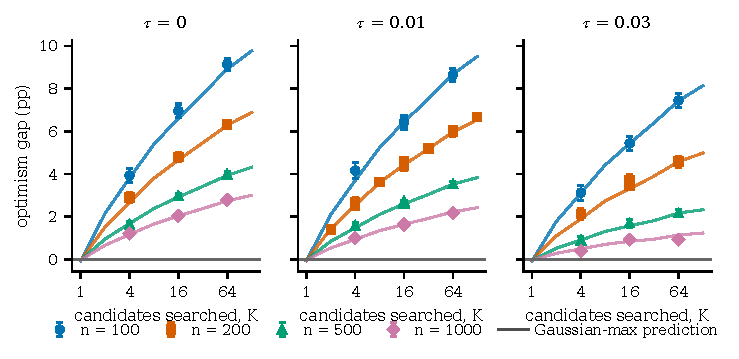
\includegraphics[width=.66\linewidth]{figures/e1_gap_vs_K_rho0.5.pdf}
\caption{Optimism gap (naive report minus exact true accuracy of the selected configuration, pp) for best-of-$K$ search against the number of candidates $K$, per tuning-set size $n$, in three panels by true spread $\tau$ ($\rho=0.5$). Markers: simulation (interaction grid, $500$ repetitions per point), bars $\pm1.96$ Monte-Carlo s.e.; lines: Gaussian-max prediction (Sec.~\ref{sec:method}). $K=1$ has no search and no gap. Over the $\N{th_cells}$ cells with both, observed minus predicted ranges from $\N{th_dmin}$ to $+\N{th_dmax}$~pp; the line extends to $K=128$, where the grid has no simulation.}\label{fig:gap}
\end{figure}

\paragraph{What drives it (Q2).}
Fig.~\ref{fig:factors} varies each factor from the reference cell. The gap is driven mainly by $n$ and $K$. A larger true spread $\tau$ lowers it ($\tau=0.03$: $\N{gap_tau003}$~pp), because a real quality difference makes the selection less noisy. Strong correlation between configurations lowers it ($\rho=0.9$: $\N{gap_rho9}$~pp vs. $\rho=0$: $\N{gap_rho0}$~pp), since correlated candidates share their noise. Generation noise raises it slightly ($\varepsilon=0.2$: $\N{gap_eps2}$~pp) and so does leakage of tuning items into the prompt, which also drives coverage down ($8$ leaked items: gap $\N{gap_leak8}$~pp, naive coverage $\N{cov_leak8}\%$). Among search procedures, successive halving has a smaller gap ($\N{gap_sh}$~pp) than best-of-$K$ and successive rejects ($\N{gap_sr}$~pp); it uses part of the data to eliminate and still reports on all of it, but its coverage is still $\N{cov_sh}\%$. The Gaussian-max prediction agrees with the simulation in the $\N{th_cells}$ cells where both exist (mean absolute difference $\N{th_meanabs}$~pp, at most $\N{th_maxabs}$~pp; $\N{th_rho5_cells}$ cells have $\rho=0.5$, and the largest simulated $K$ is $\N{th_Kmax}$, in one cell). It slightly \emph{under}predicts: the observed gap is larger in $\N{th_above}$ of $\N{th_cells}$ cells (mean difference $+\N{th_meandiff}$~pp; sign test $p\approx\N{th_signp}\times10^{-4}$), and in the $\N{th_nz}$ cells that differ by more than two combined s.e.\ it is larger in $\N{th_nz_above}$ and smaller in $\N{th_nz_below}$. We use it as an approximation, not a theorem.

\begin{figure}[tbp]
\centering
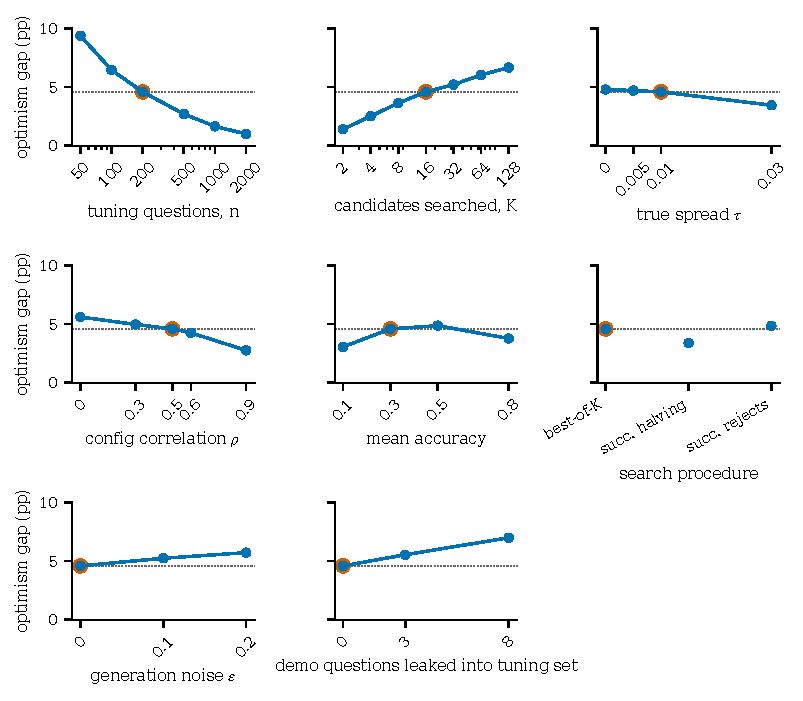
\includegraphics[width=.68\linewidth]{figures/e2_factor_effects.pdf}
\caption{Optimism gap of the naive report when one factor is varied and the others stay at the reference cell ($n=200$, $K=16$, $\tau=0.01$, $\rho=0.5$, mean accuracy $0.3$, best-of-$K$, no generation noise, no leakage; orange ring and dotted line). $2000$ repetitions per point, bars $\pm1.96$ Monte-Carlo s.e. Greedy search ran only at $K=128$ and is not comparable.}\label{fig:factors}
\end{figure}

\paragraph{Does the gap change conclusions (Q3)?}
We ask whether a method licenses the claim ``the tuned system beats the untuned baseline''. The baseline is a fixed pool configuration (index $0$, drawn like the others, chosen independently of the candidates but possibly among them by chance), scored on the same tuning items, or on the report items for the held-out split. A method \emph{claims} when (report $-$ baseline score)$/\mathrm{se}>z$, with $\mathrm{se}$ the paired standard error of the per-item difference between the selected and the baseline configuration and $z=1.645$ (one-sided $5\%$; the simultaneous critical value for the simultaneous bound). The claim is \emph{false} when the selected configuration is in truth not better than the baseline, $\mu_{\hat c}\le\mu_{\text{base}}$, and the false-claim rate is the share of claims among such repetitions ($\N{ref_nonpos}\%$ of the repetitions in the reference cell). Its null value is the boundary rate $5\%$ at $\mu_{\hat c}=\mu_{\text{base}}$; below it the rate should be lower. Requiring a true gain of $0.5$ ($1$)~pp for the claim to count as true changes the naive rate in the reference cell only to $\N{mg_naive_le05}\%$ ($\N{mg_naive_le1}\%$), and a claim with a negative true difference occurs in $\N{mg_naive_ws}\%$ of all repetitions (split: $\N{mg_split_ws}\%$, simultaneous: $\N{mg_simul_ws}\%$). A \emph{false ship} (Table~\ref{tab:ref}) is a report at least $2$~pp above the baseline's true score while the selected configuration's true score is below that bar. In the reference cell the naive report claims in $\N{ref_naive_claim}\%$ of all repetitions and in $\N{ref_naive_fp}\%$ of the false cases, against the boundary rate of $5\%$ (Fig.~\ref{fig:claims}a). With $K=128$ it does in $\N{fp_K128}\%$. The comparison of two tuned systems is equally affected when their search budgets differ (Fig.~\ref{fig:claims}b): at $\tau=0$, i.e.\ identical systems, a system tuned over $64$ configurations is claimed to beat one with a single configuration in $\N{cmp_00_6401_claim}\%$ of $\N{cmp_reps}$ repetitions, and the claim is also not true (true difference not positive) in $\N{cmp_00_6401_false}\%$ ($\N{cmp_00_6401_fc05}\%$ if a true gain of $0.5$~pp is required); the average reported difference is $\N{cmp_00_6401_diff}$~pp against a true one of about zero. With equal budgets ($16$ vs.\ $16$) the false-claim rate is $\N{cmp_00_1616_false}\%$ at $n=200$: the bias cancels when both systems were searched alike, and does not when they were not.

\begin{figure}[tbp]
\centering
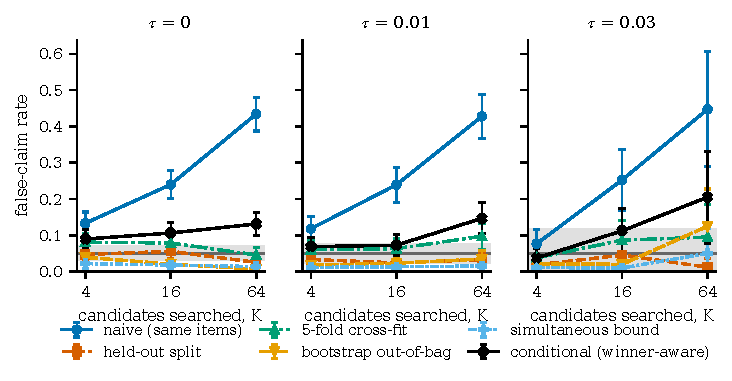
\includegraphics[width=.68\linewidth]{figures/e4_false_claims_argmax_rho0.5_n200.pdf}\\[2pt]
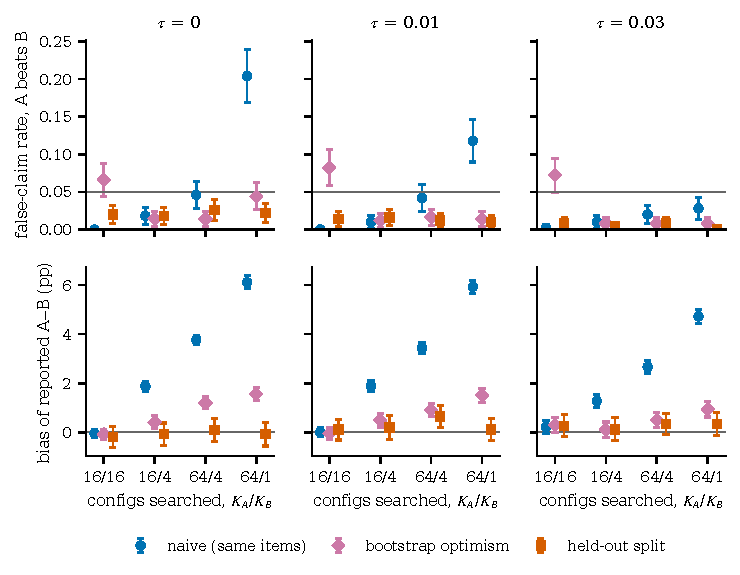
\includegraphics[width=.68\linewidth]{figures/e4_unequal_budget_n200.pdf}
\caption{(a) Share of repetitions in which a method licenses ``tuned beats untuned baseline'' (one-sided 5\%) among those where the selected configuration is truly not better ($n=200$, $\rho=0.5$, best-of-$K$; $500$ repetitions, bars $\pm1.96\sqrt{p(1-p)/m}$ with $m$ the repetitions in the denominator; the grey band is the binomial 95\% band around the nominal $0.05$). (b) Two systems tuned with $K_A$ and $K_B$ configurations, $n=200$, $500$ repetitions. Top: share of repetitions claiming ``$A$ beats $B$'' while $A$ is truly not better; line: nominal $0.05$. Bottom: bias of the reported $A-B$ difference (pp), bars $\pm1.96$ s.e.}\label{fig:claims}
\end{figure}

\paragraph{Reporting methods (Q4, Q5).}
Table~\ref{tab:ref} (Appendix~\ref{app:more}) and Fig.~\ref{fig:reliab} (Appendix~\ref{app:figs}) give bias, coverage and width in the reference cell. The study plan, written before the runs, fixes a reliability criterion that we apply to all $106$ cells and every method: $|$bias$|\le\max(2\,\text{s.e.},0.5~\text{pp})$ and 95\% coverage inside the binomial Monte-Carlo band around $0.95$. The coverage condition is two-sided, so a conservative interval fails it; we therefore also count under-coverage (below the band) and over-coverage (above it). The held-out split meets the criterion in $\N{rel_split_ok}$ of $\N{rel_split_cells}$ cells; its $\N{split_fail_bias}$ bias and $\N{split_fail_cov}$ coverage failures ($\N{rel_split_under}$ under, $\N{rel_split_over}$ over; largest $|$bias$|$ $\N{split_maxabsbias}$~pp) are of the size expected from testing $106$ cells twice at the 5\% level. It pays with half of the items (width $\N{ref_split_width}$ vs.\ $\N{ref_naive_width}$~pp; RMSE $\N{ref_split_rmse}$ vs.\ $\N{ref_naive_rmse}$~pp in the reference cell) and reports the configuration chosen from $n/2$ items, so we compare protocols at equal total items below. The naive report meets the criterion in only $\N{rel_naive_ok}$ of $106$ cells, under-covering in $\N{rel_naive_under}$. The simultaneous bound keeps the naive bias ($\N{ref_simul_bias}$~pp) but under-covers in only $\N{rel_simul_under}$ cells and over-covers in $\N{rel_simul_over}$ ($\N{ref_simul_cover}\%$ in the reference cell, width $\N{ref_simul_width}$~pp): valid and conservative. Five-fold cross-fitting under-covers in $\N{rel_crossfit_under}$ cells; the bootstrap corrections reduce the bias (out-of-bag: $\N{ref_boot_oob_bias}$~pp in the reference cell) but mostly over-cover ($\N{rel_boot_oob_over}$ over, $\N{rel_boot_oob_under}$ under), so they meet the full criterion in only $\N{rel_boot_oob_ok}$ cells. Our implementations of winner-aware conditional inference and of a hybrid interval (Appendix~\ref{app:defs}) agree with a closed form ($K=2$) and with a port of the authors' replication code, and are calibrated in exact Gaussian cases (coverage $\N{val_cov_min}$--$\N{val_cov_max}\%$). The conditional interval is nonetheless very wide in the reference cell (width $\N{ref_cond_width}$~pp; RMSE of its median $\N{ref_cond_rmse}$~pp) because the winner's lead over the truncation boundary is below $0.5$ standard errors in $\N{val_ref_lead_lt05}\%$ of repetitions. The hybrid has coverage $\N{hy_hybrid_covmin}$--$\N{hy_hybrid_covmax}\%$ at width $\N{hy_hybrid_width}$~pp ($\N{hy_simul_width}$~pp for the simultaneous bound) in the region we ran ($\rho=0.5$, mean accuracy $0.3$, $K\le64$, $\N{hy_cells}$ cells), but its point estimate is no better than the naive one. The Ladder-type report \citep{blum2015ladder} reduces the naive bias but does not remove it ($\tau=0$, $n=200$, $K=16$: $\N{lad_ladder_K16_bias}$ vs.\ $\N{lad_naive_K16_bias}$~pp).

\paragraph{Reporting protocols at equal item budgets (Q5).}
We score every protocol against the true accuracy of the configuration \emph{it} ships, at equal total items (Table~\ref{tab:fresh} in Appendix~\ref{app:more}; $\N{fr_ncells}$ combinations of $\tau\in\{0,.01,.03\}$, $K\in\{4,16,64\}$, $\rho\in\{.5,.9\}$ and $200$ or $400$ items, $\N{fr_reps}$ repetitions). A \emph{fresh-set} protocol tunes on $n_{\text{tune}}$ items, ships the winner and reports its accuracy on $m$ new items. In the reference cell with $200$ items in all, the $100/100$ fresh-set report and the $50/50$ split are unbiased ($\N{fr_fresh100_200_bias}$ and $\N{fr_split_200_bias}$~pp) with $95\%$ coverage, but their RMSE is $\N{fr_fresh100_200_rmse}$ and $\N{fr_split_200_rmse}$~pp because the report items carry their own sampling error; the best fresh allocation ($50/150$) has RMSE $\N{fr_fresh50_200_rmse}$~pp; the out-of-bag bootstrap on all $200$ items has bias $\N{fr_boot_oob_200_bias}$~pp, RMSE $\N{fr_boot_oob_200_rmse}$~pp and coverage $\N{fr_boot_oob_200_cover}\%$, the naive report $+\N{fr_naive_200_bias}$~pp and $\N{fr_naive_200_rmse}$~pp. The out-of-bag bootstrap has the smaller RMSE than the split and than the half-and-half fresh set in all $\N{fr_ncells}$ combinations, with coverage $\N{fr_oob_covmin}$--$\N{fr_oob_covmax}\%$ (conservative in most), while the hybrid's RMSE exceeds the naive one in $\N{fr_hyb_gt_naive}$. Holding items out thus buys an unbiased, assumption-free report, not a more accurate one. The out-of-bag bootstrap needs the per-item outcomes of every searched candidate and a search that can be replayed on resampled items; we checked it only for the searches here.

\paragraph{Ranking several tuned systems.}
For five systems tuned on the same items with $4$, $8$, $16$, $32$ and $64$ configurations at $\tau=0$ (all equally good, $n=200$, $\N{rk_reps}$ repetitions; Fig.~\ref{fig:rank} in Appendix~\ref{app:figs}), the naive report puts the largest-budget system first in $\N{rk_naive_big_rep}\%$ of repetitions, whereas it is truly best in $\N{rk_naive_big_true}\%$ (the held-out split: $\N{rk_split_big_rep}\%$ vs.\ $\N{rk_split_big_true}\%$); with five systems tuned alike ($16$ configurations each) the naive rate is $\N{rk_naive_eq_big_rep}\%$. When quality differs ($\tau=0.03$) the naive rank correlation with the truth is not worse than the split's (Kendall's $\tau_b$ $\N{rk_naive_kt_uneq}$ vs.\ $\N{rk_split_kt_uneq}$); the distortion is that the budget, not the quality, orders equally good systems. At an equal total budget of $400$ items the out-of-bag bootstrap, the split and the half-and-half fresh set put the $64$-candidate system first in $\N{rkb_oob_big_rep}$, $\N{rkb_split_big_rep}$ and $\N{rkb_fresh_big_rep}\%$ of repetitions at $\tau=0$ ($\N{rkb_naive_big_rep}\%$ for the naive report; truly best in $\N{rkb_big_true}\%$), so they remove the budget effect, but with true differences ($\tau=0.03$) none ranks better than the naive report by Kendall's $\tau_b$ ($\N{rkb_oob_kt}$, $\N{rkb_split_kt}$, $\N{rkb_fresh_kt}$ vs.\ $\N{rkb_naive_kt}$; $\N{rkb_reps}$ repetitions).




\subsection{Real LLM on MMLU-Pro}\label{sec:real}
\paragraph{Scale reached.} The pool is all $K=\N{real_K}$ configurations of a factorial grid of instruction wording, demonstration set and option layout, each scored on all $\N{real_items}$ items by Qwen2.5-0.5B-Instruct. Their accuracies are $\N{real_accmin}$--$\N{real_accmax}\%$ (mean $\N{real_accmean}\%$; chance $10\%$), a spread of $\N{real_sd}$~pp (s.d.), with a mean item-level correlation of $\N{real_corr}$ between configurations. This is a small-spread regime with one small model; it is not a study of large $K$, of stronger models or of DSPy or MIPRO, which we did not run. Searches are replayed on the cached $0/1$ matrix ($\N{real_reps}$ repetitions per cell). In the \emph{disjoint} arm ($n\le400$) the tuning items are drawn without replacement and the truth is the selected configuration's accuracy on the remaining $2000-n$ items; in the \emph{i.i.d.} arm they are drawn with replacement and the truth is the accuracy over the whole pool ($n\le\N{real_iid_nmax}$).

\paragraph{The gap is present and has the same shape.} With exhaustive search over the $K=\N{real_K}$ configurations the naive report exceeds the held-out accuracy of the selected configuration by $\N{real_gap_n50}\pm\N{real_gapse_n50}$~pp at $n=50$, $\N{real_gap_n100}$ at $n=100$, $\N{real_gap_n200}\pm\N{real_gapse_n200}$ at $n=200$ and $\N{real_gap_n400}$~pp at $n=400$, and the i.i.d.\ arm gives the same ($\N{real_iid_gap_n50}$, $\N{real_iid_gap_n200}$, $\N{real_iid_gap_n400}$~pp; Fig.~\ref{fig:real}). At $n=200$ it grows with the number of candidates ($K=1$: $\N{real_gap_K1_n200}\pm\N{real_gapse_K1_n200}$, $K=2$: $\N{real_gap_K2_n200}$, $K=4$: $\N{real_gap_K4_n200}$, $K=\N{real_K}$: $\N{real_gap_n200}$~pp), although the search has little to find (mean regret $\N{real_regret_n200}$~pp). At $n=200$ the cheaper searches shrink the gap but do not remove it: successive halving $\N{real_gap_sh}$~pp, greedy coordinate search over the factorial grid $\N{real_gap_greedy}$~pp, successive rejects $\N{real_gap_sr}$~pp, against $\N{real_gap_n200}$~pp for exhaustive search. The naive Wilson interval covers the truth in only $\N{real_cover_n200}\%$ of repetitions at $n=200$ ($\N{real_cover_n50}\%$ at $n=50$), and the naive report licenses ``tuned beats the baseline'' in $\N{real_fp_n200}\%$ of the repetitions at $n=200$ in which the selected configuration is truly no better ($\N{real_fp_n50}\%$ at $n=50$; nominal $5\%$).

\paragraph{The Gaussian-maximum formula and the generator, checked on the real matrix.} Fed with the empirical covariance of the real matrix, the formula of Sec.~\ref{sec:method} predicts the replayed gap at $K=\N{real_K}$ as $\N{gm_pred_n50}$ vs.\ $\N{gm_rep_n50}$~pp ($n=50$), $\N{gm_pred_n200}$ vs.\ $\N{gm_rep_n200}$ ($200$) and $\N{gm_pred_n400}$ vs.\ $\N{gm_rep_n400}$~pp ($400$; Fig.~\ref{fig:real}a); over all $\N{gm_cells}$ cells ($K\le\N{real_K}$, $n$ up to $\N{gm_nmax}$, both arms) the difference is at most $\N{gm_maxdiff}$~pp, with $\N{gm_z2}$ cells beyond two Monte-Carlo s.e. Generator settings matched to the real accuracies, mean item correlation (latent $\rho=\N{gen_rho}$) or the full pairwise correlations reproduce the real naive gap to within about ten percent (one-$\rho$ copula $\N{gen_uni_rel}\%$ on average, pairwise copula $\N{gen_tet_rel}\%$ for $K\ge4$), not exactly (Appendix~\ref{app:calib}).

\begin{figure}[tbp]
\centering
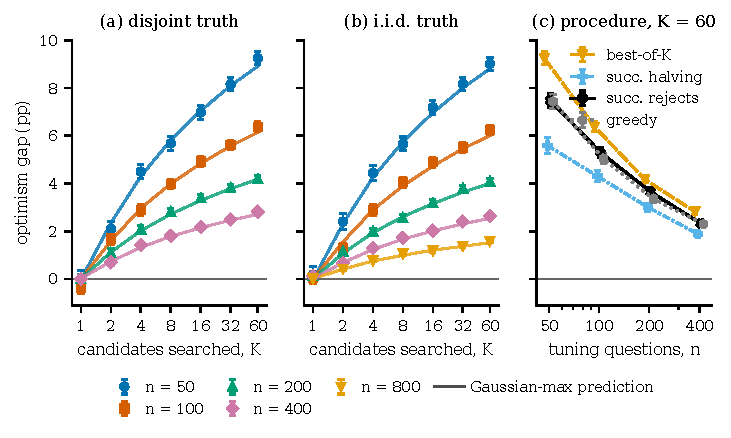
\includegraphics[width=.68\linewidth]{figures/e3_real_gap.pdf}
\caption{Real setting (Qwen2.5-0.5B-Instruct, MMLU-Pro, $K\le\N{real_K}$ complete configurations, $\N{real_reps}$ repetitions per point, bars $\pm1.96$ Monte-Carlo s.e.). Optimism gap of the naive report of best-of-$K$ search against the number of candidates searched, one colour per tuning-set size $n$; markers are the replay, lines the Gaussian-maximum prediction from the empirical covariance of the real matrix; $K=1$ is the no-search control. (a) Disjoint truth arm. (b) I.i.d.\ truth arm (truth over the whole pool). (c) At $K=\N{real_K}$, best-of-$K$, successive halving, successive rejects and greedy coordinate search against $n$ (disjoint arm).}\label{fig:real}
\end{figure}

\paragraph{Reporting methods.} Table~\ref{tab:real} (Appendix~\ref{app:more}) gives the real-setting version of the reference table. At $n=200$ the held-out split is unbiased ($\N{real_split_n200_bias}\pm\N{real_split_n200_biasse}$~pp, coverage $\N{real_split_n200_cover}\%$), the out-of-bag bootstrap reduces the bias to $\N{real_boot_oob_n200_bias}$~pp at nearly the naive width, the hybrid interval covers $\N{real_hybrid_n200_cover}\%$ with RMSE $\N{real_hybrid_n200_rmse}$~pp (naive $\N{real_naive_n200_rmse}$) and the conditional interval, $\N{real_cond_n200_width}$~pp wide, covers $\N{real_cond_n200_cover}\%$. At equal total items ($200$; Table~\ref{tab:freshreal}) the RMSE is $\N{frr_boot_oob_200_rmse}$~pp for the out-of-bag bootstrap (coverage $\N{frr_boot_oob_200_cover}\%$), $\N{frr_fresh50_200_rmse}$ and $\N{frr_fresh100_200_rmse}$~pp for $50$/$150$ and $100$/$100$ tuning/fresh items, $\N{frr_split_200_rmse}$~pp for the split and $\N{frr_naive_200_rmse}$~pp for the naive report: the order of the synthetic study.


\section{Discussion and limitations}\label{sec:discussion}
\paragraph{What to report.}
The measurements support three practices for any result obtained after an automatic search. (i)~\emph{Disclose the search}: the number of candidates, the number of tuning items, the procedure and its seeds; the synthetic gap is a function of $n$ and $K$ first (Figs.~\ref{fig:gap}, \ref{fig:factors}), and a tuned-vs-untuned or tuned-vs-tuned comparison is not like-for-like unless the budgets are given (Fig.~\ref{fig:claims}). (ii)~\emph{Report on items not used for selection when they can be spared}: select on part of the items and report on a separate set. This is unbiased and needs no modelling of the search. At equal total items it is less accurate than correcting the in-sample score (RMSE $\N{fr_fresh100_200_rmse}$~pp for $100$ tuning plus $100$ fresh items vs.\ $\N{fr_boot_oob_200_rmse}$~pp for the out-of-bag bootstrap at $200$ items, Table~\ref{tab:fresh}), so its price is accuracy, not only width. (iii)~\emph{When items cannot be spared}, either correct the score or use an interval that accounts for the selection. The out-of-bag bootstrap had the smallest error and a small bias in the synthetic reference cell and across the $\N{fr_ncells}$ equal-budget combinations (coverage $\N{fr_oob_covmin}$--$\N{fr_oob_covmax}\%$, mostly conservative), and had bias $\N{real_boot_oob_n200_bias}\pm\N{real_boot_oob_n200_biasse}$~pp, coverage $\N{real_boot_oob_n200_cover}\%$ and, at $200$ items, the smallest RMSE ($\N{frr_boot_oob_200_rmse}$ vs.\ $\N{frr_fresh100_200_rmse}$~pp for $100$/$100$ tuning/fresh items) on the real model ($K=\N{real_K}$); it requires the per-item outcomes of every candidate searched and a search that can be replayed on resampled items, which an adaptive optimiser may not allow. The hybrid winner-aware interval was near-nominal at a width near that of the simultaneous bound in the region where we ran it, but its point estimate was no better than the naive one (RMSE $\N{fr_hybrid_200_rmse}$ vs.\ $\N{fr_naive_200_rmse}$~pp at $200$ items), and the conditional interval was too wide to inform at the sample sizes studied.

\paragraph{Limitations.}
\emph{Synthetic setting.} The generator is a Gaussian copula with a finite configuration pool; its conclusions hold for that generator and the ranges of $n$, $K$, $\tau$, $\rho$ and mean accuracy we scanned (Sec.~\ref{sec:synth}), and the Gaussian-maximum prediction is an approximation that deviates by up to $0.5$~pp. On the real covariance it deviates by at most $\N{gm_maxdiff}$~pp, and a matched generator reproduces the real gap to about ten percent, not exactly (Sec.~\ref{sec:real}). \emph{Real setting.} The pool is $K=\N{real_K}$ configurations with a spread of $\N{real_sd}$~pp, a factorial grid rather than a random sample of prompts, and the searches (best-of-$K$, successive halving, successive rejects, greedy coordinate search) are replayed over that fixed pool rather than run with the LLM in the loop; a real leakage arm, a real two-system comparison and a per-subject analysis were not run, and there is no check at large $K$ and no stronger model. One small model with letter-logit scoring; the truth is the held-out remainder of a finite pool. We did not run DSPy or MIPRO and say nothing about their search dynamics. \emph{Methods.} The conditional and hybrid intervals are our implementations; they pass the checks of Appendix~\ref{app:defs} (closed form, exact-Gaussian coverage, a port of the authors' replication code) but their coverage in the data-generating setting was run only at $\rho=0.5$, mean accuracy $0.3$ and $K\le64$ for the full-evaluation argmax. The equal-budget comparison covers $200$ and $400$ items and best-of-$K$ search; the out-of-bag bootstrap was not run on adaptive search. Cross-fitting estimates the performance of the procedure run on a fraction of the data, not of the final configuration. False-claim and ranking rates depend on the claim threshold and the share of no-better configurations (varied only through $\tau$). Optimistic tuned scores can lead to deploying prompts worse than reported; correct reporting reduces that risk, and we see no direct negative use.


\bibliographystyle{plainnat}
\bibliography{refs}

\appendix
\section{Exact definitions of generators, procedures and estimators}\label{app:defs}
These definitions follow the code in \texttt{analysis/} (\texttt{synth.py}, \texttt{lib.py}, \texttt{run\_grid.py}); the table of scripts is in \texttt{REPRODUCE.md}. Throughout, $S\in\{0,1\}^{K\times n}$ holds the correctness of the $K$ candidates on the $n$ tuning items, $\hat p_c$ is the row mean, $\hat c$ the selected row, and ties in an argmax are broken at random.

\paragraph{Synthetic generator.} A pool of $128$ configurations and $N=20{,}000$ items. Configuration accuracies are $p_c=\mathrm{clip}(m+\tau z_c,0.01,0.99)$ with $z_c\sim N(0,1)$ ($m=0.3$ unless stated); an optional outlier raises one configuration's accuracy by a fixed amount. Each item has a latent $q_i\sim N(0,1)$ shared across configurations, and configuration $c$ has the latent $U_{ci}=\sqrt\rho\,q_i+\sqrt{1-\rho}\,e_{ci}$ with $e_{ci}\sim N(0,1)$; it is correct on item $i$ iff $U_{ci}<\Phi^{-1}(p_c)$, so every row has accuracy $p_c$ in expectation and any two rows have latent correlation $\rho$. The true accuracy $\mu_c$ of a configuration is its mean over the $N$ pool items (the pool is the population). A tuning set is $n$ items drawn with replacement; the $K$ candidates are drawn without replacement from the $128$ configurations. \emph{Generation noise} flips each evaluation of a candidate (and of the baseline) with probability $\varepsilon$ independently, and the truth becomes $\mu_c+\varepsilon(1-2\mu_c)$. \emph{Leakage}: each candidate shows $\ell$ tuning items with their answers in the prompt, which turns an incorrect outcome on such an item into a correct one with probability $0.9$; the truth is unchanged, and the held-out split scores its report half without leakage.

\paragraph{Search procedures.} \emph{Best-of-$K$}: $\hat c=\arg\max_c\hat p_c$ on all $n$ items. \emph{Successive halving}: $R=\lceil\log_2K\rceil$ rounds; the $n$ items are cut into $R$ consecutive blocks; in round $r$ the survivors are scored on block $r$ only and the better $\lceil|\text{alive}|/2\rceil$ stay; the report is the survivor's score on all $n$ items. \emph{Successive rejects}: budget $B=nK/4$ evaluations, $\bar\ell=\tfrac12+\sum_{i=2}^{K}1/i$; in phase $j=1,\dots,K-1$ the survivors are scored on the first $n_j=\min\{n,\max\{1,\lceil (B-K)/(\bar\ell(K+1-j))\rceil\}\}$ items and the worst is removed; the report is the winner's mean over the first $n_{K-1}$ items. \emph{Greedy coordinate ascent}: the $K$ candidates form a factorial grid ($4\times4\times4$, or $8\times4\times4$ for $K=128$); start at a random cell and, for the factors in random order, move to the best level given the others on all $n$ items, for at most $10$ sweeps; the report is the final cell's score.

\paragraph{Claim test and baseline.} The baseline is pool configuration $0$, scored on the same $n$ items as the candidates (on the report items for the held-out split), with the same generation noise. For any method with point report $\hat\theta$ and critical value $z$ ($1.645$; the simultaneous critical value $c$ for the simultaneous bound), the claim is $(\hat\theta-\hat p_{\text{base}})/\mathrm{dse}>z$, where $\mathrm{dse}$ is the standard deviation (ddof 1) of the per-item differences $S_{\hat c,i}-S_{\text{base},i}$ divided by $\sqrt{n_{\text{rep}}}$ ($n_{\text{rep}}$ the number of report items). The false-claim rate is the mean of the claim indicator over repetitions with $\mu_{\hat c}\le\mu_{\text{base}}$. A false ship is $\hat\theta\ge\mu_{\text{base}}+0.02$ and $\mu_{\hat c}<\mu_{\text{base}}+0.02$.

\paragraph{Reporting methods.} All intervals are $95\%$ ($\alpha=0.05$) and Wilson intervals use the number of items the report was computed from.
\emph{Naive}: $\hat p_{\hat c}$ with a Wilson interval on $n$. \emph{Held-out split}: the search runs on the first $\lfloor n/2\rceil$ items (the tuning set is in random order), the report is the pick's mean on the remaining items with a Wilson interval on their number. \emph{Five-fold cross-fitting}: $n$ items in five consecutive folds; for each fold the procedure runs on the other four and its pick is scored on the fold; the report is the pooled score over all $n$ items, with a Wilson interval on $n$; the configuration it describes is the full-data pick. \emph{Bootstrap}: $B=100$ resamples of the $n$ items with replacement; for each, the procedure is run on the resample, giving pick $\hat c_b$; the optimism is the score of $\hat c_b$ on the resample minus its score on the original items, and the optimism-corrected report is the naive score minus the mean optimism; the out-of-bag report is the mean score of $\hat c_b$ on the items absent from resample $b$; the $.632$ report is $0.368\,\hat p_{\hat c}+0.632\,\text{OOB}$; intervals are the report $\pm1.96\sqrt{\hat\theta(1-\hat\theta)/n}$, i.e.\ they ignore the selection. \emph{Simultaneous bound}: $B=300$ bootstrap resamples of the items; $c$ is the $0.95$ quantile of $\max_k|\hat p^*_k-\hat p_k|/\mathrm{se}_k$ with $\mathrm{se}_k=\sqrt{\max(\hat p_k(1-\hat p_k),10^{-4})/n}$; the interval is $\hat p_{\hat c}\pm c\,\mathrm{se}_{\hat c}$ and the point report is naive. \emph{Ladder}: $\eta=1/\sqrt n$; candidates are visited in a random order; the first sets the ladder value $\mathrm{round}(\hat p/\eta)\eta$, a later one replaces the selected configuration and the value only if $\hat p>\text{value}+\eta$; the report is the final value with a Wilson interval on $n$.

\paragraph{Conditional and hybrid intervals.} Both treat $\hat p\sim N(\mu,\hat\Sigma/n)$ with $\hat\Sigma$ the sample covariance of the rows of $S$, and apply to best-of-$K$ only. To remove lattice ties each score is dithered by one uniform draw on $\pm1/(2n)$ per repetition, used for every quantity of that repetition, which leaves the argmax a random-tie argmax. Given the winner $\hat c=k$, the event $\{\hat c=k\}$ is a polyhedron in $\hat p_k$ once the component of $\hat p$ orthogonal to $\hat p_k$ is fixed (the polyhedral lemma of \citet{lee2016exact}, in the form for the winner of a maximum \citep{andrews2024winners}); its truncation interval $[V^-,V^+]$ is computed from the $K-1$ contrasts. \emph{Conditional}: the conditional law of $\hat p_k$ is $N(\theta,\sigma_k^2)$ truncated to $[V^-,V^+]$; the estimate is the $\theta$ at which the conditional CDF at the observed value equals $1/2$ and the interval endpoints are the $\theta$ at which it equals $1-\alpha/2$ and $\alpha/2$ (root-finding on $\hat p_k\pm80\sigma_k$). \emph{Hybrid}: $\beta=0.005$; $c_\beta$ is the $1-\beta$ quantile (from $1000$ Monte-Carlo draws) of $\max_j|Z_j|$ with $Z\sim N(0,\text{corr}(\hat\Sigma))$; for each $\theta_0$ on a grid of $161$ values in $\hat p_k\pm c_\beta\sigma_k$ the truncation interval is intersected with $[\theta_0-c_\beta\sigma_k,\theta_0+c_\beta\sigma_k]$, and $\theta_0$ is retained if the conditional CDF of $\hat p_k$ lies in $[a_1,1-a_1]$ with $a_1=(\alpha-\beta)/(2(1-\beta))$; the interval is the range of retained values and the point estimate is the median of the truncated normal on the restricted set (the hybrid median-unbiased estimate, always within $\hat p_k\pm c_\beta\sigma_k$). The conditional point estimate is the unrestricted conditional median.
\emph{Validation.} (1) For $K=2$ the conditional CDF equals an independent closed form (computed with mpmath) to $\N{val_k2_cdf}$ over $2000$ draws. (2) With exact Gaussian draws and known $\Sigma$ ($\N{val_ncases}$ cases, $K=2$--$16$, $\tau$ from $0$ to $.05$, $n$ from $200$ to $1000$, $3000$ repetitions) the probability-integral transform of the conditional CDF at the true score is uniform (Kolmogorov--Smirnov $p$-values $\N{val_ks_min}$--$\N{val_ks_max}$) and both intervals cover $\N{val_cov_min}$--$\N{val_cov_max}\%$. (3) A Python port of the authors' MATLAB replication code for the conditional and hybrid routines agrees on $\N{val_akm_n}$ random covariance matrices ($\N{val_akm_skip}$ more were skipped because the port's truncated-normal quantile saturates): truncation limits to $10^{-12}$, conditional limits and median to about $10^{-6}$ standard errors, hybrid limits to within one step of our $161$-point grid (the port uses $4001$ points) and the hybrid median to $0.04$ of a step. (4) In the reference cell with known $\Sigma$ the conditional interval covers $\N{val_ref_cond_cov_known}\%$ (with $\Sigma$ estimated from Bernoulli draws: $\N{val_ref_cond_cov_est}\%$), with mean width $\N{val_ref_cond_width_mean}$ and median width $\N{val_ref_cond_width_med}$~pp.

\paragraph{Real replay.} The correctness matrix $Y\in\{0,1\}^{K\times2000}$ is fixed. Each repetition draws $n$ items without replacement as the tuning set (candidates are all $K$ complete configurations, or a random subset), runs a procedure and a reporting method on them, and takes as truth the selected configuration's accuracy on the other $2000-n$ items. The baseline for claims is the hand-written default (instruction $0$, demonstration set $1$, plain layout; accuracy $19.15\%$), which is one of the candidates when all $K$ are searched. Greedy coordinate search is run on the $6\times5\times2$ grid of instruction, demonstration set and layout (all $60$ configurations), with the same random start and sweeps as in the synthetic study. In the i.i.d. arm the $n$ items are drawn with replacement and the truth is the accuracy of the selected configuration on all $2000$ items. The Gaussian-maximum prediction for the real matrix uses $\epsilon\sim\mathcal N(0,\hat\Sigma/n)$ with $\hat\Sigma$ the empirical covariance of the $0/1$ item matrix of the $K$ candidates ($5000$ draws). In the disjoint arm the truth is the accuracy on the $N-n$ remaining items ($N=2000$), so the tuning noise has covariance $(1-n/N)\hat\Sigma/n$ and the predicted gap is $N/(N-n)$ times the expected noise of the selected configuration. The generator matched to the real matrix (Appendix~\ref{app:calib}) uses the real accuracies as thresholds of a Gaussian copula with either one latent correlation or the pairwise tetrachoric correlation matrix of the real $0/1$ data (eigenvalues clipped to be positive semi-definite)..

\section{Further reporting-method results}\label{app:more}
The other methods mostly fail the criterion, for different reasons. The naive report fails in all but $\N{rel_naive_ok}$ of $106$ cells, under-covering in $\N{rel_naive_under}$. The simultaneous bound keeps the naive bias ($\N{ref_simul_bias}$~pp) but under-covers in only $\N{rel_simul_under}$ cells and over-covers in $\N{rel_simul_over}$ ($\N{ref_simul_cover}\%$ in the reference cell), at a width of $\N{ref_simul_width}$~pp: it is valid and conservative. Five-fold cross-fitting has bias near zero in $\N{rel_crossfit_okb}$ cells but under-covers in $\N{rel_crossfit_under}$ ($\N{ref_crossfit_cover}\%$ in the reference cell) because its interval ignores the variance added by selection. The bootstrap optimism correction reduces the bias from $\N{ref_naive_bias}$ to $\N{ref_boot_opt_bias}$~pp and its out-of-bag variant to $\N{ref_boot_oob_bias}$~pp (bias criterion met in $\N{rel_boot_oob_okb}$ cells) but over-covers in $\N{rel_boot_oob_over}$ cells ($\N{ref_boot_oob_cover}\%$ in the reference cell) and under-covers in $\N{rel_boot_oob_under}$, so it meets the full criterion in only $\N{rel_boot_oob_ok}$ of $106$. Our implementation of winner-aware conditional inference was run in $\N{rel_cond_cells}$ cells; it covers correctly in the reference cell ($\N{ref_cond_cover}\%$) and is outside the band in $\N{rel_cond_under}$ (under) and $\N{rel_cond_over}$ (over) of them, but its intervals are very wide ($\N{ref_cond_width}$~pp), its heavy-tailed conditional median has RMSE $\N{ref_cond_rmse}$~pp and it meets the bias criterion in $\N{rel_cond_okb}$ of them. The instability is not a coding fault (Appendix~\ref{app:defs}): the conditional median is median-unbiased, but when the winner's standardised lead over the truncation boundary is small the truncated normal is nearly flat over a long left tail in the score, so the mean error is large. In the reference cell with known $\Sigma$ the lead is below $0.5$ standard errors in $\N{val_ref_lead_lt05}\%$ of repetitions (median $\N{val_ref_lead_med}$); in the $\N{lead_ref_share_small}\%$ with a lead below $0.25$ the conditional median has median error $\N{lead_ref_condmed_err}$~pp and mean error $\N{lead_ref_condmean_err}$~pp and its interval has median width $\N{lead_ref_condwidth_med}$~pp, while the hybrid has mean error $\N{lead_ref_hyberr}$~pp at width $\N{lead_ref_hybwidth}$~pp. Over all repetitions the point-estimate RMSE is $\N{val_ref_cond_rmse}$~pp for the conditional and $\N{val_ref_hyb_rmse}$~pp for the hybrid median (median absolute error $\N{val_ref_cond_medae}$ and $\N{val_ref_hyb_medae}$~pp). With one clearly better configuration ($+5$~pp, $K=16$, $n=500$) the winner is the truly best in $\N{lead_clear_n500_best}\%$ of repetitions ($\N{lead_clear_n1000_best}\%$ at $n=1000$, where the conditional interval is $\N{lead_clear_n1000_width}$~pp wide, as wide as the naive one). The conditional interval is thus a correct but uninformative answer when the data barely separate the winner from the rest. A hybrid interval of the same family (projection interval plus the conditional test on the restricted truncation set) has coverage $\N{hy_hybrid_covmin}$--$\N{hy_hybrid_covmax}\%$ at a mean width of $\N{hy_hybrid_width}$~pp over $\N{hy_cells}$ cells of the $\tau\times n\times K$ grid ($\N{hy_reps}$ repetitions each; Fig.~\ref{fig:hybrid} in Appendix~\ref{app:figs}), against $\N{hy_naive_covmin}$--$\N{hy_naive_covmax}\%$ at $\N{hy_naive_width}$~pp for the naive interval and $\N{hy_simul_covmin}$--$\N{hy_simul_covmax}\%$ at $\N{hy_simul_width}$~pp for the simultaneous bound. It needs the full-evaluation argmax and a Gaussian approximation and was checked only at $\rho=0.5$, mean accuracy $0.3$ and $K\le64$; we do not recommend it for its point estimate. The Ladder-type report \citep{blum2015ladder} (sequential submission) reduces the naive bias but does not remove it ($\tau=0$, $n=200$, $K=16$: $\N{lad_ladder_K16_bias}$ vs.\ $\N{lad_naive_K16_bias}$~pp).

\begin{table}[h]
\centering
\caption{Reporting methods in the reference cell, exact truth. Every row is scored against the true accuracy of the configuration it reports on: the selected configuration for all rows except the held-out split, which reports on the configuration chosen from $n/2$ items (Table~\ref{tab:fresh} compares protocols at equal total items).}\label{tab:ref}
{\footnotesize\setlength{\tabcolsep}{3.5pt}
\begin{tabular}{lrrrrrr}
\toprule
method & bias (pp) & RMSE (pp) & coverage & width (pp) & false claim & false ship \\
\midrule
naive (same items) & $4.59 \pm 0.06$ & 5.25 & $0.759 \pm 0.010$ & 13.1 & 0.248 & 0.818 \\
held-out split & $0.07 \pm 0.11$ & 4.72 & $0.946 \pm 0.005$ & 17.6 & 0.036 & 0.327 \\
5-fold cross-fit & $0.00 \pm 0.09$ & 4.23 & $0.866 \pm 0.008$ & 12.6 & 0.070 & 0.278 \\
bootstrap optimism & $1.27 \pm 0.06$ & 3.14 & $0.966 \pm 0.004$ & 13.2 & 0.051 & 0.356 \\
bootstrap out-of-bag & $-0.09 \pm 0.06$ & 2.86 & $0.974 \pm 0.004$ & 12.7 & 0.017 & 0.207 \\
bootstrap .632 & $1.63 \pm 0.06$ & 3.18 & $0.960 \pm 0.004$ & 12.9 & 0.058 & 0.411 \\
simultaneous bound & $4.57 \pm 0.06$ & 5.25 & $0.983 \pm 0.003$ & 19.4 & 0.012 & 0.818 \\
conditional (winner-aware) & $-10.45 \pm 0.87$ & 40.45 & $0.952 \pm 0.005$ & 60.5 & 0.091 & 0.354 \\
\bottomrule
\end{tabular}}

\par\smallskip\begin{minipage}{.97\linewidth}\footnotesizeReference cell: n=200, K=16, $\tau$=.01, $\rho$=.5, mean accuracy .3, best-of-K; 2000 repetitions. Bias and coverage are mean $\pm$ Monte Carlo s.e.; coverage is of the nominal 95\% interval for the true score of the selected configuration; false claim: rate of claiming tuned $>$ baseline when it is not truly better; false ship: rate of reporting a score at least 2 pp above the baseline's true score while the selected configuration's true score is below that bar.
\end{minipage}
\end{table}

\begin{table}[h]
\centering
\caption{Reporting protocols at equal total items, each scored against its own shipped configuration (reference cell).}\label{tab:fresh}
{\footnotesize\setlength{\tabcolsep}{3.5pt}
\begin{tabular}{lrrrrrr}
\toprule
protocol & items & true acc. (\%) & bias (pp) & RMSE (pp) & coverage & width (pp) \\
\midrule
naive & 200 & 30.44 & $4.53 \pm 0.10$ & 5.19 & $0.762 \pm 0.017$ & 13.1 \\
bootstrap out-of-bag & 200 & 30.46 & $-0.12 \pm 0.12$ & 2.85 & $0.975 \pm 0.006$ & 12.7 \\
bootstrap optimism & 200 & 30.46 & $1.23 \pm 0.12$ & 3.13 & $0.958 \pm 0.008$ & 13.2 \\
simultaneous bound & 200 & 30.45 & $4.51 \pm 0.10$ & 5.18 & $0.970 \pm 0.007$ & 19.4 \\
5-fold cross-fit & 200 & 30.48 & $-0.04 \pm 0.18$ & 4.42 & $0.848 \pm 0.015$ & 12.6 \\
hybrid (proj.+cond.) & 200 & 30.44 & $-0.88 \pm 0.23$ & 5.63 & $0.940 \pm 0.010$ & 16.5 \\
held-out split 50/50 & 200 & 30.29 & $-0.02 \pm 0.19$ & 4.57 & $0.952 \pm 0.009$ & 17.6 \\
fresh set 50/150 & 200 & 30.20 & $-0.04 \pm 0.16$ & 3.87 & $0.940 \pm 0.010$ & 14.5 \\
fresh set 100/100 & 200 & 30.34 & $-0.23 \pm 0.18$ & 4.53 & $0.952 \pm 0.009$ & 17.6 \\
\midrule
naive & 400 & 30.59 & $3.16 \pm 0.08$ & 3.66 & $0.788 \pm 0.017$ & 9.2 \\
bootstrap out-of-bag & 400 & 30.57 & $-0.06 \pm 0.08$ & 2.07 & $0.973 \pm 0.007$ & 9.0 \\
bootstrap optimism & 400 & 30.57 & $0.91 \pm 0.08$ & 2.26 & $0.962 \pm 0.008$ & 9.3 \\
simultaneous bound & 400 & 30.57 & $3.18 \pm 0.07$ & 3.67 & $0.978 \pm 0.006$ & 13.7 \\
5-fold cross-fit & 400 & 30.57 & $0.14 \pm 0.12$ & 2.98 & $0.862 \pm 0.014$ & 9.0 \\
hybrid (proj.+cond.) & 400 & 30.58 & $-0.36 \pm 0.16$ & 4.00 & $0.950 \pm 0.009$ & 11.5 \\
held-out split 50/50 & 400 & 30.42 & $0.17 \pm 0.14$ & 3.34 & $0.928 \pm 0.011$ & 12.6 \\
fresh set 100/300 & 400 & 30.30 & $0.16 \pm 0.10$ & 2.54 & $0.950 \pm 0.009$ & 10.3 \\
fresh set 200/200 & 400 & 30.46 & $0.26 \pm 0.12$ & 2.99 & $0.960 \pm 0.008$ & 12.7 \\
\bottomrule
\end{tabular}}

\par\smallskip\begin{minipage}{.97\linewidth}\footnotesizeReference cell ($\tau$=.01, $K$=16, $\rho$=.5, mean accuracy .3, best-of-$K$), 600 repetitions; the budget (items) is the total number of questions consumed: methods above the fresh-set rows tune and report on the same items (in-sample), a fresh-set row ``$n_{\rm tune}/m$'' tunes on $n_{\rm tune}$ items and reports the winner on $m$ new items (Wilson interval). Each row is scored against its own truth, the true accuracy of the configuration that protocol shipped (third column; it differs across protocols because the search saw different data). Bias and coverage are mean $\pm$ Monte Carlo s.e.; coverage is of the nominal 95\% interval; the held-out split tunes on one half of the items and reports on the other.
\end{minipage}
\end{table}

\begin{table}[h]
\centering
\caption{Reporting methods in the real setting (best-of-$K$ with $K=\N{real_K}$ complete configurations, disjoint truth).}\label{tab:real}
{\footnotesize\setlength{\tabcolsep}{3.5pt}
\begin{tabular}{rlrrrr}
\toprule
$n$ & method & bias (pp) & RMSE (pp) & coverage & width (pp) \\
\midrule
50 & naive (same items) & $9.25 \pm 0.13$ & 10.19 & $0.641 \pm 0.015$ & 24.0 \\
 & held-out split & $-0.15 \pm 0.24$ & 7.57 & $0.960 \pm 0.006$ & 28.6 \\
 & 5-fold cross-fit & $0.17 \pm 0.21$ & 6.73 & $0.896 \pm 0.010$ & 20.8 \\
 & bootstrap optimism & $2.56 \pm 0.15$ & 5.40 & $0.985 \pm 0.004$ & 24.7 \\
 & bootstrap out-of-bag & $-0.17 \pm 0.14$ & 4.50 & $0.978 \pm 0.005$ & 21.2 \\
 & bootstrap .632 & $3.30 \pm 0.14$ & 5.48 & $0.978 \pm 0.005$ & 22.7 \\
 & simultaneous bound & $9.27 \pm 0.13$ & 10.20 & $0.995 \pm 0.002$ & 38.6 \\
 & conditional (winner-aware) & $-25.69 \pm 2.64$ & 87.26 & $0.964 \pm 0.006$ & 130.4 \\
 & hybrid (proj.+cond.) & $-1.51 \pm 0.32$ & 10.20 & $0.971 \pm 0.005$ & 32.4 \\
\midrule
200 & naive (same items) & $4.18 \pm 0.07$ & 4.80 & $0.709 \pm 0.014$ & 11.6 \\
 & held-out split & $-0.07 \pm 0.13$ & 4.00 & $0.944 \pm 0.007$ & 15.0 \\
 & 5-fold cross-fit & $-0.09 \pm 0.12$ & 3.76 & $0.843 \pm 0.012$ & 10.7 \\
 & bootstrap optimism & $0.97 \pm 0.08$ & 2.80 & $0.964 \pm 0.006$ & 11.6 \\
 & bootstrap out-of-bag & $-0.32 \pm 0.08$ & 2.61 & $0.966 \pm 0.006$ & 10.7 \\
 & bootstrap .632 & $1.34 \pm 0.08$ & 2.83 & $0.952 \pm 0.007$ & 11.1 \\
 & simultaneous bound & $4.17 \pm 0.08$ & 4.80 & $0.988 \pm 0.003$ & 18.4 \\
 & conditional (winner-aware) & $-11.04 \pm 1.23$ & 40.50 & $0.953 \pm 0.007$ & 56.2 \\
 & hybrid (proj.+cond.) & $-0.85 \pm 0.16$ & 5.19 & $0.966 \pm 0.006$ & 15.3 \\
\bottomrule
\end{tabular}}

\par\smallskip\begin{minipage}{.97\linewidth}\footnotesizeReal-LLM replay on MMLU-Pro with Qwen2.5-0.5B-Instruct: best-of-$K$ over the $K$=60 configurations, tuning set of $n$ questions drawn without replacement from the 2000-question pool; 1000 repetitions per row. Truth = accuracy of the selected configuration on the pool questions outside the tuning set (finite-pool truth). Bias and coverage are mean $\pm$ Monte Carlo s.e.; coverage is of the nominal 95\% interval. The bias and RMSE of the conditional method are dominated by the heavy tail of its estimate (reported as measured).
\end{minipage}
\end{table}

\begin{table}[h]
\centering
\caption{Reporting protocols at equal total items on the real matrix, each scored against its own shipped configuration.}\label{tab:freshreal}
{\footnotesize\setlength{\tabcolsep}{3.5pt}
\begin{tabular}{lrrrrrr}
\toprule
protocol & items & true acc. (\%) & bias (pp) & RMSE (pp) & coverage & width (pp) \\
\midrule
naive & 200 & 18.82 & $4.46 \pm 0.11$ & 5.10 & $0.650 \pm 0.021$ & 11.6 \\
bootstrap out-of-bag & 200 & 18.81 & $-0.05 \pm 0.12$ & 2.74 & $0.944 \pm 0.010$ & 10.8 \\
bootstrap optimism & 200 & 18.81 & $1.23 \pm 0.12$ & 3.00 & $0.956 \pm 0.009$ & 11.7 \\
simultaneous bound & 200 & 18.83 & $4.45 \pm 0.11$ & 5.09 & $0.986 \pm 0.005$ & 18.4 \\
5-fold cross-fit & 200 & 18.81 & $0.08 \pm 0.16$ & 3.65 & $0.856 \pm 0.016$ & 10.7 \\
hybrid (proj.+cond.) & 200 & 18.82 & $-0.46 \pm 0.22$ & 4.99 & $0.966 \pm 0.008$ & 15.4 \\
held-out split 50/50 & 200 & 18.54 & $0.08 \pm 0.18$ & 3.91 & $0.948 \pm 0.010$ & 15.0 \\
fresh set 50/150 & 200 & 18.46 & $-0.04 \pm 0.15$ & 3.36 & $0.936 \pm 0.011$ & 12.3 \\
fresh set 100/100 & 200 & 18.58 & $0.05 \pm 0.17$ & 3.76 & $0.950 \pm 0.010$ & 15.0 \\
\bottomrule
\end{tabular}}

\par\smallskip\begin{minipage}{.97\linewidth}\footnotesizeReal-LLM replay on MMLU-Pro (Qwen2.5-0.5B-Instruct), best-of-$K$ with $K$=60 configurations (largest $K$ in the file), total budget 200 questions, 500 repetitions. Questions are drawn without replacement from the 2000-question pool; each row is scored against the accuracy of the configuration it shipped on the pool questions that protocol did not use (third column, true accuracy of the shipped configuration). Columns as in the synthetic table.
\end{minipage}
\end{table}

\section{Additional synthetic results}\label{app:tables}
\begin{table}[h]
\centering
\caption{Naive optimism gap by tuning-set size and number of candidates.}\label{tab:gapnk}
{\footnotesize\setlength{\tabcolsep}{3.5pt}
\begin{tabular}{rrrrr}
\toprule
$\tau$ & $n$ & $K$=4 & $K$=16 & $K$=64 \\
\midrule
0 & 100 & $3.92 \pm 0.17$ & $6.96 \pm 0.16$ & $9.14 \pm 0.14$ \\
0 & 200 & $2.90 \pm 0.12$ & $4.81 \pm 0.10$ & $6.32 \pm 0.10$ \\
0 & 500 & $1.65 \pm 0.08$ & $2.97 \pm 0.07$ & $3.98 \pm 0.07$ \\
0 & 1000 & $1.22 \pm 0.05$ & $2.04 \pm 0.05$ & $2.80 \pm 0.05$ \\
\midrule
0.03 & 100 & $3.13 \pm 0.18$ & $5.44 \pm 0.16$ & $7.44 \pm 0.16$ \\
0.03 & 200 & $2.12 \pm 0.13$ & $3.72 \pm 0.12$ & $4.58 \pm 0.13$ \\
0.03 & 500 & $0.90 \pm 0.08$ & $1.70 \pm 0.09$ & $2.18 \pm 0.09$ \\
0.03 & 1000 & $0.40 \pm 0.06$ & $0.93 \pm 0.06$ & $0.92 \pm 0.06$ \\
\bottomrule
\end{tabular}}

\par\smallskip\begin{minipage}{.97\linewidth}\footnotesizeNaive optimism gap (pp; reported minus true score of the selected configuration), mean $\pm$ Monte Carlo s.e. over 500 repetitions; $\rho$=.5, best-of-K.
\end{minipage}
\end{table}
\begin{table}[h]
\centering
\caption{Stress cells.}\label{tab:stress}
{\footnotesize\setlength{\tabcolsep}{3.5pt}
\begin{tabular}{llrrrr}
\toprule
cell & method & bias (pp) & coverage & width (pp) & false claim \\
\midrule
$n$=50, $K$=128, acc. 0.1 & naive (same items) & $10.41 \pm 0.08$ & $0.330 \pm 0.011$ & 21.9 & 0.550 \\
 & held-out split & $0.15 \pm 0.13$ & $0.967 \pm 0.004$ & 23.7 & 0.056 \\
 & 5-fold cross-fit & $0.07 \pm 0.13$ & $0.908 \pm 0.006$ & 16.5 & 0.060 \\
 & bootstrap out-of-bag & $0.04 \pm 0.07$ & $0.990 \pm 0.002$ & 16.5 & 0.004 \\
 & simultaneous bound & $10.40 \pm 0.08$ & $0.999 \pm 0.001$ & 41.9 & 0.000 \\
 & conditional (winner-aware) & $-28.54 \pm 1.83$ & $0.965 \pm 0.004$ & 138.5 & 0.117 \\
\midrule
$n$=200, $K$=16, outl. 0.03 & naive (same items) & $4.74 \pm 0.05$ & $0.757 \pm 0.010$ & 13.1 & 0.257 \\
 & held-out split & $-0.09 \pm 0.10$ & $0.949 \pm 0.005$ & 17.6 & 0.042 \\
 & 5-fold cross-fit & $0.08 \pm 0.09$ & $0.867 \pm 0.008$ & 12.6 & 0.085 \\
 & bootstrap out-of-bag & $0.01 \pm 0.06$ & $0.975 \pm 0.003$ & 12.7 & 0.025 \\
 & simultaneous bound & $4.74 \pm 0.06$ & $0.973 \pm 0.004$ & 19.4 & 0.015 \\
 & conditional (winner-aware) & $-10.23 \pm 0.83$ & $0.950 \pm 0.005$ & 62.3 & 0.104 \\
\midrule
$n$=200, $K$=128, outl. 0.03 & naive (same items) & $6.88 \pm 0.05$ & $0.409 \pm 0.011$ & 13.3 & 0.535 \\
 & held-out split & $-0.04 \pm 0.10$ & $0.953 \pm 0.005$ & 17.6 & 0.034 \\
 & 5-fold cross-fit & $-0.02 \pm 0.09$ & $0.875 \pm 0.007$ & 12.6 & 0.082 \\
 & bootstrap out-of-bag & $-0.13 \pm 0.06$ & $0.988 \pm 0.002$ & 12.7 & 0.016 \\
 & simultaneous bound & $6.87 \pm 0.05$ & $0.986 \pm 0.003$ & 23.5 & 0.014 \\
 & conditional (winner-aware) & $-13.07 \pm 0.97$ & $0.957 \pm 0.005$ & 77.5 & 0.150 \\
\midrule
$n$=200, $K$=16, outl. 0.05 & naive (same items) & $4.59 \pm 0.06$ & $0.767 \pm 0.009$ & 13.1 & 0.252 \\
 & held-out split & $-0.01 \pm 0.10$ & $0.955 \pm 0.005$ & 17.6 & 0.042 \\
 & 5-fold cross-fit & $0.02 \pm 0.09$ & $0.875 \pm 0.007$ & 12.6 & 0.082 \\
 & bootstrap out-of-bag & $-0.14 \pm 0.06$ & $0.975 \pm 0.003$ & 12.7 & 0.022 \\
 & simultaneous bound & $4.58 \pm 0.06$ & $0.983 \pm 0.003$ & 19.4 & 0.015 \\
 & conditional (winner-aware) & $-9.78 \pm 0.82$ & $0.966 \pm 0.004$ & 61.0 & 0.094 \\
\midrule
$n$=200, $K$=128, outl. 0.05 & naive (same items) & $6.10 \pm 0.07$ & $0.505 \pm 0.011$ & 13.3 & 0.546 \\
 & held-out split & $0.08 \pm 0.10$ & $0.951 \pm 0.005$ & 17.7 & 0.041 \\
 & 5-fold cross-fit & $-0.31 \pm 0.10$ & $0.846 \pm 0.008$ & 12.7 & 0.082 \\
 & bootstrap out-of-bag & $-0.76 \pm 0.07$ & $0.939 \pm 0.005$ & 12.8 & 0.017 \\
 & simultaneous bound & $6.08 \pm 0.07$ & $0.981 \pm 0.003$ & 23.6 & 0.014 \\
 & conditional (winner-aware) & $-13.77 \pm 1.04$ & $0.953 \pm 0.005$ & 72.8 & 0.152 \\
\bottomrule
\end{tabular}}

\par\smallskip\begin{minipage}{.97\linewidth}\footnotesizeStress cells ($\tau$=0, $\rho$=.5, best-of-K; outlier = fraction of outlier configurations); 2000 repetitions each. Columns as in the reference-cell table (RMSE and false-ship rate omitted for width; they are in the results file); bias and coverage are mean $\pm$ Monte Carlo s.e.; outl. = outlier-configuration fraction, acc. = mean accuracy (.3 unless shown).
\end{minipage}
\end{table}
\begin{table}[h]
\centering
\caption{Two tuned systems with unequal search budgets.}\label{tab:unequal}
{\footnotesize\setlength{\tabcolsep}{3.5pt}
\begin{tabular}{rlrrrrrr}
\toprule
$\tau$ & $K_A/K_B$ & claim (naive) & false claim & wrong sign & reported diff. (pp) & true diff. (pp) & false claim (split) \\
\midrule
0 & 16/16 & $0.000 \pm 0.000$ & 0.000 & 0.000 & -0.05 & 0.01 & 0.020 \\
0 & 16/4 & $0.034 \pm 0.008$ & 0.018 & 0.018 & 1.84 & -0.04 & 0.018 \\
0 & 64/4 & $0.114 \pm 0.014$ & 0.046 & 0.046 & 3.77 & 0.01 & 0.026 \\
0 & 64/1 & $0.492 \pm 0.022$ & 0.204 & 0.202 & 6.17 & 0.06 & 0.022 \\
\midrule
0.01 & 16/16 & $0.000 \pm 0.000$ & 0.000 & 0.000 & -0.02 & -0.01 & 0.014 \\
0.01 & 16/4 & $0.038 \pm 0.009$ & 0.010 & 0.010 & 2.16 & 0.28 & 0.016 \\
0.01 & 64/4 & $0.122 \pm 0.015$ & 0.042 & 0.042 & 3.82 & 0.38 & 0.012 \\
0.01 & 64/1 & $0.532 \pm 0.022$ & 0.118 & 0.118 & 6.74 & 0.81 & 0.010 \\
\midrule
0.03 & 16/16 & $0.016 \pm 0.006$ & 0.002 & 0.002 & 0.33 & 0.12 & 0.008 \\
0.03 & 16/4 & $0.130 \pm 0.015$ & 0.010 & 0.010 & 2.75 & 1.48 & 0.004 \\
0.03 & 64/4 & $0.318 \pm 0.021$ & 0.020 & 0.020 & 5.16 & 2.49 & 0.008 \\
0.03 & 64/1 & $0.736 \pm 0.020$ & 0.028 & 0.028 & 8.99 & 4.27 & 0.000 \\
\bottomrule
\end{tabular}}

\par\smallskip\begin{minipage}{.97\linewidth}\footnotesizeTwo tuned systems A and B searched with $K_A$ and $K_B$ configurations (best-of-K, $n$=200); 500 repetitions per row. Naive columns: claim = rate of claiming A$>$B (one-sided 5\%), false claim = claim while A is truly not better (true difference $\le$ 0), wrong sign = claim while A is truly worse; mean reported and true difference A$-$B in pp. Last column: false-claim rate of the held-out split.
\end{minipage}
\end{table}

\section{Additional figures}\label{app:figs}
Figures~\ref{fig:hybrid}--\ref{fig:reliab} support the reporting-methods paragraph and the ranking paragraph of Sec.~\ref{sec:synth}; their numbers are in the result files named in \texttt{REPRODUCE.md}.
\begin{figure}[tbp]
\centering
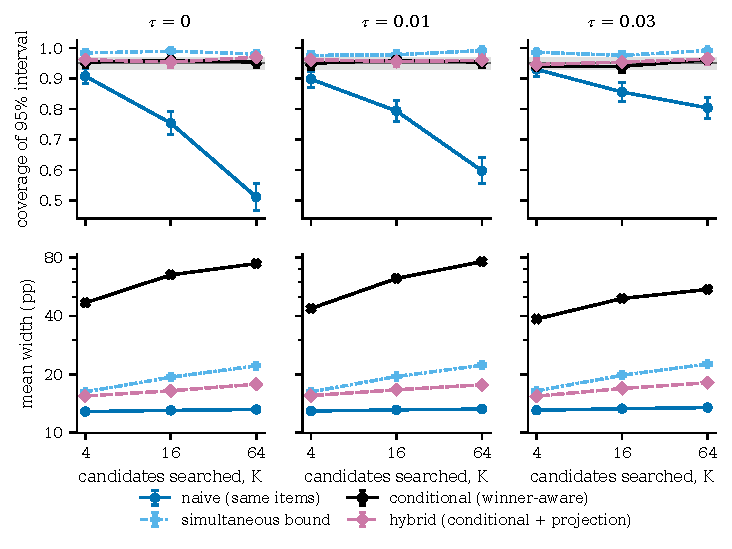
\includegraphics[width=\linewidth]{figures/e5b_hybrid_n200.pdf}
\caption{Winner-aware intervals for the argmax winner ($n=200$, $\rho=0.5$, $500$ repetitions). Coverage of the nominal 95\% interval for the true score of the selected configuration (bars $\pm1.96$ s.e.; grey band: binomial Monte-Carlo band) and mean width (log scale) for the naive, simultaneous, conditional and hybrid intervals.}\label{fig:hybrid}
\end{figure}


\begin{figure}[tbp]
\centering
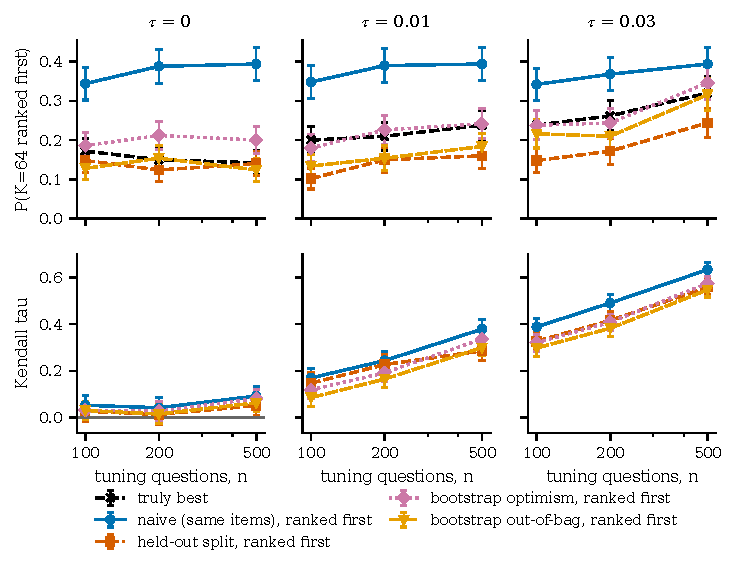
\includegraphics[width=\linewidth]{figures/e4c_ranking.pdf}
\caption{Ranking five systems tuned on the same items with $K=4,8,16,32,64$ configurations (best-of-$K$, $500$ repetitions). Top: share of repetitions in which each method ranks the $K=64$ system first, against how often it is truly best (black dashed). Bottom: mean Kendall's $\tau$ between reported and true ranking.}\label{fig:rank}
\end{figure}

\begin{figure}[tbp]
\centering
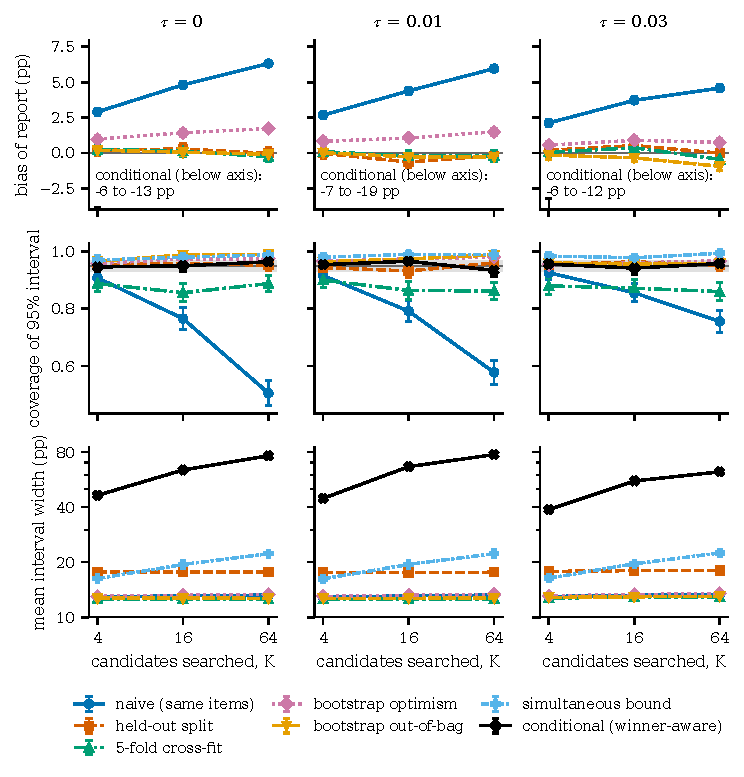
\includegraphics[width=\linewidth]{figures/e5_reliability_argmax_rho0.5_n200.pdf}
\caption{Reporting methods against the exact truth ($n=200$, $\rho=0.5$, best-of-$K$, $500$ repetitions). Top: bias of the reported score. Middle: coverage of the nominal 95\% interval (grey band: binomial 95\% Monte-Carlo band). Bottom: mean interval width (log scale). The conditional method lies below the plotted bias range (see panel text) and has intervals $40$--$80$~pp wide.}\label{fig:reliab}
\end{figure}

\section{Generator calibrated to the real matrix}\label{app:calib}
To check that the synthetic generator is informative about real tuned scores, we built generator settings that match the real matrix and compared their naive gap with the real replay (Table~\ref{tab:calib}). Both settings use the $\N{real_K}$ real accuracies as the configuration accuracies and as the thresholds of a Gaussian copula over items: (i) one common latent correlation, chosen ($\rho=\N{gen_rho}$) to reproduce the mean pairwise $\varphi$ of the real $0/1$ matrix; (ii) the full matrix of pairwise tetrachoric correlations of the real data ($\N{gen_clip}$ eigenvalues clipped to make it positive semi-definite). Each generator is run on $10$ pools of $2000$ items with $300$ repetitions each, with the replay procedure of the real study. Mean accuracy, the spread of accuracies, the dispersion of item difficulty (standard deviation across items of the share of configurations solving the item: $\N{gen_sditem_real}$ real, $\N{gen_sditem_gen}$ generator) and the mean $\varphi$ are matched by the one-$\rho$ copula (the pairwise copula shares the thresholds). The one-$\rho$ copula cannot reproduce the heterogeneity of the pairwise $\varphi$ (real $\N{gen_phi_min}$--$\N{gen_phi_max}$; largest pairwise error $\N{gen_pw_err_uni}$) and overstates the gap at $K\ge4$; the pairwise copula matches every pair (largest error $\N{gen_pw_err_tet}$) and understates it slightly, probably through higher-order structure that a Gaussian copula does not carry. At mean accuracy $0.195$, latent $\rho=0.3,0.5,0.7,0.9$ correspond to an observed $\varphi$ of $\N{phimap_3},\N{phimap_5},\N{phimap_7},\N{phimap_9}$; the real $\varphi=\N{gen_phi_real}$ lies between the grid values $\rho=0.5$ and $0.9$ of the synthetic study, and the grid's mean accuracy of $0.3$ instead of $0.18$ changes $\varphi$ at equal $\rho$ by about $0.03$ ($\N{phimap_m3_r5}$ vs.\ $\N{phimap_5}$ at $\rho=0.5$). Over all $\N{gen_uni_cells}$ cells ($K=1,\dots,\N{real_K}$, $n$ up to $\N{gm_nmax}$, both arms) the one-$\rho$ copula differs from the replay by more than two Monte-Carlo s.e. in $\N{gen_uni_z2}$ cells and the pairwise copula in $\N{gen_tet_z2}$.
\begin{table}[h]
\centering
\caption{Generator calibrated to the real matrix against the real replay.}\label{tab:calib}
{\footnotesize\setlength{\tabcolsep}{3.5pt}
\begin{tabular}{lrrr}
\toprule
quantity & real matrix & one-rho copula & pairwise copula \\
\midrule
accuracy, mean (\%) & 18.23 & 18.21 & (same thresholds) \\
accuracy, sd across configs (pp) & 1.16 & 1.17 & (same thresholds) \\
item difficulty, sd across items & 0.232 & 0.231 & -- \\
mean pairwise $\phi$ & 0.348 & 0.344 & -- \\
pairwise $\phi$, min--max & $-$0.007--0.926 & 0.321--0.366 & -- \\
pairwise $\phi$, max $|\Delta|$ over pairs & -- & 0.572 & 0.053 \\
\midrule
naive gap, $n$=200, $K$=2 (pp) & $1.09 \pm 0.09$ & $1.14 \pm 0.05$ (+0.5) & $1.09 \pm 0.05$ ($-$0.0) \\
naive gap, $n$=200, $K$=4 (pp) & $2.07 \pm 0.08$ & $2.04 \pm 0.05$ ($-$0.4) & $1.97 \pm 0.05$ ($-$1.1) \\
naive gap, $n$=200, $K$=8 (pp) & $2.81 \pm 0.08$ & $2.95 \pm 0.05$ (+1.5) & $2.67 \pm 0.05$ ($-$1.6) \\
naive gap, $n$=200, $K$=16 (pp) & $3.39 \pm 0.08$ & $3.57 \pm 0.04$ (+2.1) & $3.31 \pm 0.05$ ($-$0.9) \\
naive gap, $n$=200, $K$=32 (pp) & $3.81 \pm 0.08$ & $4.30 \pm 0.04$ (+5.6) & $3.83 \pm 0.05$ (+0.2) \\
naive gap, $n$=200, $K$=60 (pp) & $4.18 \pm 0.07$ & $4.85 \pm 0.04$ (+7.8) & $4.14 \pm 0.04$ ($-$0.4) \\
\midrule
generator $-$ real, mean ($K\ge4$, \%) & -- & $+6.8$ & $-1.3$ \\
generator $-$ real, range ($K\ge4$, \%) & -- & $-10$ to $+16$ & $-14$ to $+4$ \\
cells with $|z|>2$ & -- & 31 of 63 & 4 of 63 \\
\bottomrule
\end{tabular}}

\par\smallskip\begin{minipage}{.97\linewidth}\footnotesizeGaussian-copula generator calibrated to the real matrix (accuracies as thresholds): one common latent correlation (``one-rho'', matched to the mean pairwise $\phi$) or one per pair (``pairwise copula'', tetrachoric correlations, 19 eigenvalues clipped). Gap rows: disjoint truth arm, mean $\pm$ s.e. (pp) of the generator (10 pools $\times$ 300 replications) with $z$ against the real replay in parentheses. Summary rows pool all $n$ (50, 100, 200, 400, 800) and both truth arms (disjoint and iid). The copula cannot reproduce the heterogeneity of the real pairwise dependence (near-duplicate and near-independent pairs) and, for the pairwise version, higher-order structure.
\end{minipage}
\end{table}

\section{Real-LLM setup and compute record}\label{app:setup}
Table~\ref{tab:setup} records the model, data revision, scoring protocol and compute of the real-LLM study as read from the committed compute log.
\begin{table}[h]
\centering
\caption{Setup and compute record of the real-LLM study (read from the compute log).}\label{tab:setup}
{\footnotesize\setlength{\tabcolsep}{3.5pt}
\begin{tabular}{lp{0.64\linewidth}}
\toprule
item & value \\
\midrule
model & Qwen2.5-0.5B-Instruct, fp32, CPU; option-letter log-probabilities \\
benchmark & MMLU-Pro test, revision \texttt{b189ec765aa7}, 2000 questions (seed 2024) \\
configurations & 60 complete of 60 planned (instruction wording $\times$ demo set $\times$ layout) \\
forward passes & 120,000 scored of 120,000 planned \\
accuracy across configs & mean 18.2\%, range 15.2--20.8\%, sd 1.16 pp \\
item correlation & mean pairwise correlation of item correctness across configs 0.35 \\
scoring jobs & 10 scoring jobs of 6 configurations each, all finished; wall-clock 20.7--34.7 h per job (0.7 h for the job resumed after an out-of-memory stop) \\
replay jobs & real replay K=60 disjoint (argmax/sh/sr/greedy), M=1000 85 min; real replay K=60 iid, M=1000 109 min \\
seeds & configs/demos 12345, questions 2024, replay 5 \\
packages & Python 3.11.2, numpy 2.4.6, scipy 1.17.1, pandas 3.0.6, scikit-learn 1.9.1, torch 2.14.1+cpu, transformers 5.22.1 \\
\bottomrule
\end{tabular}}

\par\smallskip\begin{minipage}{.97\linewidth}\footnotesizeSetup and compute record of the real-LLM matrix, from the compute log and the matrix summary; all 60 planned configurations are scored. Scoring wall-clock is elapsed time in the job on a shared host and includes time the container was frozen, so it exceeds the CPU time used. Replay times are the logged running times.
\end{minipage}
\end{table}


\section*{NeurIPS Paper Checklist}



\begin{enumerate}

\item {\bf Claims}
    \item[] Question: Do the main claims made in the abstract and introduction accurately reflect the paper's contributions and scope?
    \item[] Answer: \answerYes{}
    \item[] Justification: Abstract and introduction state the synthetic findings with their ranges, and say that the real-LLM part is a replay of searches over $K=\N{real_K}$ configurations of one small model and that DSPy/MIPRO were not run (Secs.~\ref{sec:intro}, \ref{sec:synth}, \ref{sec:real}).
    \item[] Guidelines:
    \begin{itemize}
        \item The answer \answerNA{} means that the abstract and introduction do not include the claims made in the paper.
        \item The abstract and/or introduction should clearly state the claims made, including the contributions made in the paper and important assumptions and limitations. A \answerNo{} or \answerNA{} answer to this question will not be perceived well by the reviewers. 
        \item The claims made should match theoretical and experimental results, and reflect how much the results can be expected to generalize to other settings. 
        \item It is fine to include aspirational goals as motivation as long as it is clear that these goals are not attained by the paper. 
    \end{itemize}

\item {\bf Limitations}
    \item[] Question: Does the paper discuss the limitations of the work performed by the authors?
    \item[] Answer: \answerYes{}
    \item[] Justification: Section~\ref{sec:discussion} lists the limits (synthetic generator, one small model and a finite pool, the reduced K, our own implementations of conditional/hybrid inference, validation ranges of the hybrid interval).
    \item[] Guidelines:
    \begin{itemize}
        \item The answer \answerNA{} means that the paper has no limitation while the answer \answerNo{} means that the paper has limitations, but those are not discussed in the paper. 
        \item The authors are encouraged to create a separate ``Limitations'' section in their paper.
        \item The paper should point out any strong assumptions and how robust the results are to violations of these assumptions (e.g., independence assumptions, noiseless settings, model well-specification, asymptotic approximations only holding locally). The authors should reflect on how these assumptions might be violated in practice and what the implications would be.
        \item The authors should reflect on the scope of the claims made, e.g., if the approach was only tested on a few datasets or with a few runs. In general, empirical results often depend on implicit assumptions, which should be articulated.
        \item The authors should reflect on the factors that influence the performance of the approach. For example, a facial recognition algorithm may perform poorly when image resolution is low or images are taken in low lighting. Or a speech-to-text system might not be used reliably to provide closed captions for online lectures because it fails to handle technical jargon.
        \item The authors should discuss the computational efficiency of the proposed algorithms and how they scale with dataset size.
        \item If applicable, the authors should discuss possible limitations of their approach to address problems of privacy and fairness.
        \item While the authors might fear that complete honesty about limitations might be used by reviewers as grounds for rejection, a worse outcome might be that reviewers discover limitations that aren't acknowledged in the paper. The authors should use their best judgment and recognize that individual actions in favor of transparency play an important role in developing norms that preserve the integrity of the community. Reviewers will be specifically instructed to not penalize honesty concerning limitations.
    \end{itemize}

\item {\bf Theory assumptions and proofs}
    \item[] Question: For each theoretical result, does the paper provide the full set of assumptions and a complete (and correct) proof?
    \item[] Answer: \answerNA{}
    \item[] Justification: The paper has no theorems; the Gaussian-maximum gap formula (Sec.~\ref{sec:method}) is used only as an empirical approximation and compared with simulation.
    \item[] Guidelines:
    \begin{itemize}
        \item The answer \answerNA{} means that the paper does not include theoretical results. 
        \item All the theorems, formulas, and proofs in the paper should be numbered and cross-referenced.
        \item All assumptions should be clearly stated or referenced in the statement of any theorems.
        \item The proofs can either appear in the main paper or the supplemental material, but if they appear in the supplemental material, the authors are encouraged to provide a short proof sketch to provide intuition. 
        \item Inversely, any informal proof provided in the core of the paper should be complemented by formal proofs provided in appendix or supplemental material.
        \item Theorems and Lemmas that the proof relies upon should be properly referenced. 
    \end{itemize}

    \item {\bf Experimental result reproducibility}
    \item[] Question: Does the paper fully disclose all the information needed to reproduce the main experimental results of the paper to the extent that it affects the main claims and/or conclusions of the paper (regardless of whether the code and data are provided or not)?
    \item[] Answer: \answerYes{}
    \item[] Justification: Generators, pool construction, procedures, reporting methods and settings are specified in Sec.~\ref{sec:method}; seeds, versions, commands and the figure/table-to-script map are in the reproduction notes (\texttt{REPRODUCE.md}) shipped with the code.
    \item[] Guidelines:
    \begin{itemize}
        \item The answer \answerNA{} means that the paper does not include experiments.
        \item If the paper includes experiments, a \answerNo{} answer to this question will not be perceived well by the reviewers: Making the paper reproducible is important, regardless of whether the code and data are provided or not.
        \item If the contribution is a dataset and\slash or model, the authors should describe the steps taken to make their results reproducible or verifiable. 
        \item Depending on the contribution, reproducibility can be accomplished in various ways. For example, if the contribution is a novel architecture, describing the architecture fully might suffice, or if the contribution is a specific model and empirical evaluation, it may be necessary to either make it possible for others to replicate the model with the same dataset, or provide access to the model. In general. releasing code and data is often one good way to accomplish this, but reproducibility can also be provided via detailed instructions for how to replicate the results, access to a hosted model (e.g., in the case of a large language model), releasing of a model checkpoint, or other means that are appropriate to the research performed.
        \item While NeurIPS does not require releasing code, the conference does require all submissions to provide some reasonable avenue for reproducibility, which may depend on the nature of the contribution. For example
        \begin{enumerate}
            \item If the contribution is primarily a new algorithm, the paper should make it clear how to reproduce that algorithm.
            \item If the contribution is primarily a new model architecture, the paper should describe the architecture clearly and fully.
            \item If the contribution is a new model (e.g., a large language model), then there should either be a way to access this model for reproducing the results or a way to reproduce the model (e.g., with an open-source dataset or instructions for how to construct the dataset).
            \item We recognize that reproducibility may be tricky in some cases, in which case authors are welcome to describe the particular way they provide for reproducibility. In the case of closed-source models, it may be that access to the model is limited in some way (e.g., to registered users), but it should be possible for other researchers to have some path to reproducing or verifying the results.
        \end{enumerate}
    \end{itemize}


\item {\bf Open access to data and code}
    \item[] Question: Does the paper provide open access to the data and code, with sufficient instructions to faithfully reproduce the main experimental results, as described in supplemental material?
    \item[] Answer: \answerYes{}
    \item[] Justification: MMLU-Pro is public at a pinned revision and the code, cached correctness matrix and result files ship with the submission; the notes give the exact commands (a public link is withheld for anonymity).
    \item[] Guidelines:
    \begin{itemize}
        \item The answer \answerNA{} means that paper does not include experiments requiring code.
        \item Please see the NeurIPS code and data submission guidelines (\url{https://neurips.cc/public/guides/CodeSubmissionPolicy}) for more details.
        \item While we encourage the release of code and data, we understand that this might not be possible, so \answerNo{} is an acceptable answer. Papers cannot be rejected simply for not including code, unless this is central to the contribution (e.g., for a new open-source benchmark).
        \item The instructions should contain the exact command and environment needed to run to reproduce the results. See the NeurIPS code and data submission guidelines (\url{https://neurips.cc/public/guides/CodeSubmissionPolicy}) for more details.
        \item The authors should provide instructions on data access and preparation, including how to access the raw data, preprocessed data, intermediate data, and generated data, etc.
        \item The authors should provide scripts to reproduce all experimental results for the new proposed method and baselines. If only a subset of experiments are reproducible, they should state which ones are omitted from the script and why.
        \item At submission time, to preserve anonymity, the authors should release anonymized versions (if applicable).
        \item Providing as much information as possible in supplemental material (appended to the paper) is recommended, but including URLs to data and code is permitted.
    \end{itemize}


\item {\bf Experimental setting/details}
    \item[] Question: Does the paper specify all the training and test details (e.g., data splits, hyperparameters, how they were chosen, type of optimizer) necessary to understand the results?
    \item[] Answer: \answerYes{}
    \item[] Justification: Tuning-set size, number of candidates, procedures, splits and the unit of repetition are given in Sec.~\ref{sec:method} and the experiments; nothing is trained, and the model is used for deterministic scoring only.
    \item[] Guidelines:
    \begin{itemize}
        \item The answer \answerNA{} means that the paper does not include experiments.
        \item The experimental setting should be presented in the core of the paper to a level of detail that is necessary to appreciate the results and make sense of them.
        \item The full details can be provided either with the code, in appendix, or as supplemental material.
    \end{itemize}

\item {\bf Experiment statistical significance}
    \item[] Question: Does the paper report error bars suitably and correctly defined or other appropriate information about the statistical significance of the experiments?
    \item[] Answer: \answerYes{}
    \item[] Justification: Every reported rate, bias and coverage carries a Monte-Carlo standard error or binomial band over thousands of whole-pipeline repetitions (repetition counts in captions); coverage is compared with the binomial band, and the true spread of cells is reported.
    \item[] Guidelines:
    \begin{itemize}
        \item The answer \answerNA{} means that the paper does not include experiments.
        \item The authors should answer \answerYes{} if the results are accompanied by error bars, confidence intervals, or statistical significance tests, at least for the experiments that support the main claims of the paper.
        \item The factors of variability that the error bars are capturing should be clearly stated (for example, train/test split, initialization, random drawing of some parameter, or overall run with given experimental conditions).
        \item The method for calculating the error bars should be explained (closed form formula, call to a library function, bootstrap, etc.)
        \item The assumptions made should be given (e.g., Normally distributed errors).
        \item It should be clear whether the error bar is the standard deviation or the standard error of the mean.
        \item It is OK to report 1-sigma error bars, but one should state it. The authors should preferably report a 2-sigma error bar than state that they have a 96\% CI, if the hypothesis of Normality of errors is not verified.
        \item For asymmetric distributions, the authors should be careful not to show in tables or figures symmetric error bars that would yield results that are out of range (e.g., negative error rates).
        \item If error bars are reported in tables or plots, the authors should explain in the text how they were calculated and reference the corresponding figures or tables in the text.
    \end{itemize}

\item {\bf Experiments compute resources}
    \item[] Question: For each experiment, does the paper provide sufficient information on the computer resources (type of compute workers, memory, time of execution) needed to reproduce the experiments?
    \item[] Answer: \answerYes{}
    \item[] Justification: Compute (CPU only, no GPU) is stated in \texttt{REPRODUCE.md}: scoring jobs, running times and CPU-hours from the compute log; the synthetic grid runs in the stated time on CPU.
    \item[] Guidelines:
    \begin{itemize}
        \item The answer \answerNA{} means that the paper does not include experiments.
        \item The paper should indicate the type of compute workers CPU or GPU, internal cluster, or cloud provider, including relevant memory and storage.
        \item The paper should provide the amount of compute required for each of the individual experimental runs as well as estimate the total compute. 
        \item The paper should disclose whether the full research project required more compute than the experiments reported in the paper (e.g., preliminary or failed experiments that didn't make it into the paper). 
    \end{itemize}
    
\item {\bf Code of ethics}
    \item[] Question: Does the research conducted in the paper conform, in every respect, with the NeurIPS Code of Ethics \url{https://neurips.cc/public/EthicsGuidelines}?
    \item[] Answer: \answerYes{}
    \item[] Justification: The work uses public data and a public model, involves no human subjects, and follows the NeurIPS Code of Ethics; the limits of the claims are stated.
    \item[] Guidelines:
    \begin{itemize}
        \item The answer \answerNA{} means that the authors have not reviewed the NeurIPS Code of Ethics.
        \item If the authors answer \answerNo, they should explain the special circumstances that require a deviation from the Code of Ethics.
        \item The authors should make sure to preserve anonymity (e.g., if there is a special consideration due to laws or regulations in their jurisdiction).
    \end{itemize}


\item {\bf Broader impacts}
    \item[] Question: Does the paper discuss both potential positive societal impacts and negative societal impacts of the work performed?
    \item[] Answer: \answerYes{}
    \item[] Justification: Broader impact is discussed in Sec.~\ref{sec:discussion}: optimistic tuned scores can mislead deployment, and the paper offers corrective reporting; we see no direct negative use.
    \item[] Guidelines:
    \begin{itemize}
        \item The answer \answerNA{} means that there is no societal impact of the work performed.
        \item If the authors answer \answerNA{} or \answerNo, they should explain why their work has no societal impact or why the paper does not address societal impact.
        \item Examples of negative societal impacts include potential malicious or unintended uses (e.g., disinformation, generating fake profiles, surveillance), fairness considerations (e.g., deployment of technologies that could make decisions that unfairly impact specific groups), privacy considerations, and security considerations.
        \item The conference expects that many papers will be foundational research and not tied to particular applications, let alone deployments. However, if there is a direct path to any negative applications, the authors should point it out. For example, it is legitimate to point out that an improvement in the quality of generative models could be used to generate Deepfakes for disinformation. On the other hand, it is not needed to point out that a generic algorithm for optimizing neural networks could enable people to train models that generate Deepfakes faster.
        \item The authors should consider possible harms that could arise when the technology is being used as intended and functioning correctly, harms that could arise when the technology is being used as intended but gives incorrect results, and harms following from (intentional or unintentional) misuse of the technology.
        \item If there are negative societal impacts, the authors could also discuss possible mitigation strategies (e.g., gated release of models, providing defenses in addition to attacks, mechanisms for monitoring misuse, mechanisms to monitor how a system learns from feedback over time, improving the efficiency and accessibility of ML).
    \end{itemize}
    
\item {\bf Safeguards}
    \item[] Question: Does the paper describe safeguards that have been put in place for responsible release of data or models that have a high risk for misuse (e.g., pre-trained language models, image generators, or scraped datasets)?
    \item[] Answer: \answerNA{}
    \item[] Justification: The paper releases no model or data with a high risk of misuse; the cached correctness matrix contains only 0/1 outcomes and option log-probabilities on a public benchmark.
    \item[] Guidelines:
    \begin{itemize}
        \item The answer \answerNA{} means that the paper poses no such risks.
        \item Released models that have a high risk for misuse or dual-use should be released with necessary safeguards to allow for controlled use of the model, for example by requiring that users adhere to usage guidelines or restrictions to access the model or implementing safety filters. 
        \item Datasets that have been scraped from the Internet could pose safety risks. The authors should describe how they avoided releasing unsafe images.
        \item We recognize that providing effective safeguards is challenging, and many papers do not require this, but we encourage authors to take this into account and make a best faith effort.
    \end{itemize}

\item {\bf Licenses for existing assets}
    \item[] Question: Are the creators or original owners of assets (e.g., code, data, models), used in the paper, properly credited and are the license and terms of use explicitly mentioned and properly respected?
    \item[] Answer: \answerYes{}
    \item[] Justification: MMLU-Pro (MIT license, pinned revision) and Qwen2.5-0.5B-Instruct (Apache-2.0) are cited and used within their licenses; related methods are cited in Sec.~\ref{sec:related}.
    \item[] Guidelines:
    \begin{itemize}
        \item The answer \answerNA{} means that the paper does not use existing assets.
        \item The authors should cite the original paper that produced the code package or dataset.
        \item The authors should state which version of the asset is used and, if possible, include a URL.
        \item The name of the license (e.g., CC-BY 4.0) should be included for each asset.
        \item For scraped data from a particular source (e.g., website), the copyright and terms of service of that source should be provided.
        \item If assets are released, the license, copyright information, and terms of use in the package should be provided. For popular datasets, \url{paperswithcode.com/datasets} has curated licenses for some datasets. Their licensing guide can help determine the license of a dataset.
        \item For existing datasets that are re-packaged, both the original license and the license of the derived asset (if it has changed) should be provided.
        \item If this information is not available online, the authors are encouraged to reach out to the asset's creators.
    \end{itemize}

\item {\bf New assets}
    \item[] Question: Are new assets introduced in the paper well documented and is the documentation provided alongside the assets?
    \item[] Answer: \answerYes{}
    \item[] Justification: The code, the correctness matrix and the result files are new assets documented in \texttt{REPRODUCE.md} and the code README; they are provided anonymously with the submission.
    \item[] Guidelines:
    \begin{itemize}
        \item The answer \answerNA{} means that the paper does not release new assets.
        \item Researchers should communicate the details of the dataset\slash code\slash model as part of their submissions via structured templates. This includes details about training, license, limitations, etc. 
        \item The paper should discuss whether and how consent was obtained from people whose asset is used.
        \item At submission time, remember to anonymize your assets (if applicable). You can either create an anonymized URL or include an anonymized zip file.
    \end{itemize}

\item {\bf Crowdsourcing and research with human subjects}
    \item[] Question: For crowdsourcing experiments and research with human subjects, does the paper include the full text of instructions given to participants and screenshots, if applicable, as well as details about compensation (if any)? 
    \item[] Answer: \answerNA{}
    \item[] Justification: The research involved no crowdsourcing and no human subjects.
    \item[] Guidelines:
    \begin{itemize}
        \item The answer \answerNA{} means that the paper does not involve crowdsourcing nor research with human subjects.
        \item Including this information in the supplemental material is fine, but if the main contribution of the paper involves human subjects, then as much detail as possible should be included in the main paper. 
        \item According to the NeurIPS Code of Ethics, workers involved in data collection, curation, or other labor should be paid at least the minimum wage in the country of the data collector. 
    \end{itemize}

\item {\bf Institutional review board (IRB) approvals or equivalent for research with human subjects}
    \item[] Question: Does the paper describe potential risks incurred by study participants, whether such risks were disclosed to the subjects, and whether Institutional Review Board (IRB) approvals (or an equivalent approval/review based on the requirements of your country or institution) were obtained?
    \item[] Answer: \answerNA{}
    \item[] Justification: The research involved no human subjects, so no IRB approval was needed.
    \item[] Guidelines:
    \begin{itemize}
        \item The answer \answerNA{} means that the paper does not involve crowdsourcing nor research with human subjects.
        \item Depending on the country in which research is conducted, IRB approval (or equivalent) may be required for any human subjects research. If you obtained IRB approval, you should clearly state this in the paper. 
        \item We recognize that the procedures for this may vary significantly between institutions and locations, and we expect authors to adhere to the NeurIPS Code of Ethics and the guidelines for their institution. 
        \item For initial submissions, do not include any information that would break anonymity (if applicable), such as the institution conducting the review.
    \end{itemize}

\item {\bf Declaration of LLM usage}
    \item[] Question: Does the paper describe the usage of LLMs if it is an important, original, or non-standard component of the core methods in this research? Note that if the LLM is used only for writing, editing, or formatting purposes and does \emph{not} impact the core methodology, scientific rigor, or originality of the research, declaration is not required.
    %this research? 
    \item[] Answer: \answerYes{}
    \item[] Justification: The LLM under tuning (Qwen2.5-0.5B-Instruct, fp32, deterministic letter-logit scoring) is described in Secs.~\ref{sec:method} and \ref{sec:real}; the study, code and text were produced by AI agents under human-specified tasks, as stated in \texttt{REPRODUCE.md}, and no agent is listed as an author.
    \item[] Guidelines:
    \begin{itemize}
        \item The answer \answerNA{} means that the core method development in this research does not involve LLMs as any important, original, or non-standard components.
        \item Please refer to our LLM policy in the NeurIPS handbook for what should or should not be described.
    \end{itemize}

\end{enumerate}

\end{document}
